\documentclass{scrbook}

\usepackage{natbib}
\usepackage{graphicx}
\usepackage{amsthm}
\usepackage{amsmath}
\usepackage{color}
\usepackage{lmodern}
\usepackage{sidecap}
\usepackage[scaled]{helvet}

\renewcommand*\familydefault{\sfdefault} %% Only if the base font of the document is to be sans serif
\usepackage[T1]{fontenc}
\linespread{1.5}

\title{Demonstrating Quantum Speed-Up with a 2 Transmon Quantum Processor.}
\author{Andreas Dewes}

\theoremstyle{definition}
\newtheorem{theorem}{Theorem}[chapter]
\newtheorem{axiom}{Axiom}[theorem]

\newcommand{\bracket}[1]{\left< #1 \right>} % for Dirac brackets
\newcommand{\ket}[1]{\left| #1 \right>} % for Dirac bras
\newcommand{\bra}[1]{\left< #1 \right|} % for Dirac kets
\newcommand{\todo}[1]{\marginpar{\textcolor{red}{To Do: #1}}}
\newcommand{\figcomment}[1]{\textcolor{red}{Comment: #1}}
\newcommand{\comment}[1]{\marginpar{\textcolor{green}{To Do: #1}}}
\newcommand{\advisorcomment}[1]{\marginpar{\textcolor{yellow}{To Do: #1}}}

\begin{document}

\maketitle

\tableofcontents

\listoffigures

\listoftables

\chapter{Introduction \& Summary}

%Provide a short summary of the whole PhD thesis:
% -Introduction to QC & CQED
% -Building Blocks of Superconducting Quantum Processors
% -Realization of a Two-Transmon QP
% -Tune-Up & Characterization of the Universal Two-Qubit Gate
% -Grover's Algorithm: Introduction & Background
% -Implementation on the Two-Qubit Processor
% -Design of a Scalable QC Architecture

\section{Quantum Computing \& Circuit Quantum Electrodynamics}

\begin{figure}
	\centering
		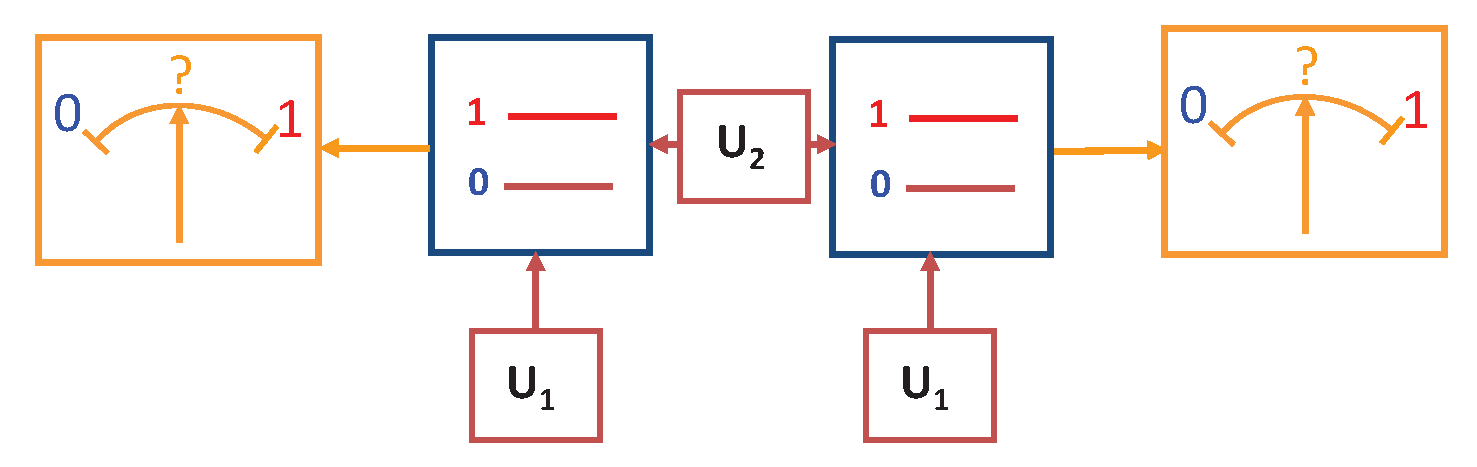
\includegraphics[width=0.8\textwidth]{./material/papers/grover/submission1/Fig1}
	\caption[Blueprint of a two-qubit quantum processor]{The blueprint of a two-qubit quantum processor. Shown are two qubits that can be individually manipulated ($U_1$) and are connected by a universal two-qubit gate $U_2$. Each of the qubits can be read out individually.}
	\label{fig:qubit_processor_blueprint}
\end{figure}

This thesis presents experiments performed with a superconducting two-qubit quantum processor. The main goal of this work was to demonstrate a possible quantum computing architecture using superconducting qubits that follows the canonical blueprint of a quantum processor as shown in fig. \ref{fig:qubit_processor_blueprint}, following the four criteria formulated by \cite{divincenzo_physical_2000}. Following this definition, a universal quantum computer is a register of quantum bits -- or qubits -- on which one can perform universal single- and two-qubit quantum gates, read out the state of each qubit individually and with high fidelity and reset the qubit register to a well-defined state.

Implementing this allegedly simple list of requirements in a system of superconducting qubits has been a major research challenge during the last decade. The first demonstration of coherent quantum dynamics in a superconducting charge-based qubit by \cite{nakamura_coherent_1999} opened up a broad research field on superconducting quantum bits. In the years following Nakamuras initial experiment, several types of superconducting qubits were proposed and realized using e.g. the superconducting phase \citep{martinis_energy-level_1985,martinis_rabi_2002} across a Josephson junction or the magnetic flux \citep{mooij_josephson_1999,chiorescu_coherent_2003} inside a superconducting ring interrupted by one or several Josephson junctions as the dominant quantum variable. An important result on the way to the development of robust superconducting qubits was the development of the so-called {\it Quantronium} qubit by \cite{vion_manipulating_2002}, which achieved quantum-mechanical coherence times larger than 1 $\mu s$, made possible by operating a Cooper pair box at a sweet spot in a regime where the charging and Josephson phase energies of the system are of comparable value. The high coherence times achieved with this qubit made it possible to perform --for the first time-- robust, NMR-like quantum operations using a superconducting qubit \citep{collin_nmr-like_2004}. Then, in 2004, the development of a new type of qubit, the so called {\it Transmon} by \cite{wallraff_strong_2004} marked again a drastic improvement in coherence times. By decreasing the charging energy of a Cooper pair box and thus operating the device in the phase regime, the resulting qubit becomes quasi insensitive to charge noise. Furthermore, by embedding the Transmon qubit in a superconducting coplanar waveguide (CPW) resonator it is possible to protect it from external sources of electrical noise and to use the dirspersive interaction between the qubit and the resonator for reading out the qubit state\citep{blais_cavity_2004}. With this so-called {\it circuit quantum electrodyanmics} (CQED) architecture, quantum gates and algorithms with up to three qubits have been implemented so-far, demonstrating multi-qubit entanglement \citep{dicarlo_preparation_2010} and simple quantum algorithms \citep{dicarlo_demonstration_2009}.

\todo{Think about moving the section on 3D-CQED directly after this one since this would probably be more logical}

In parallel to this, the development of reliable quantum-limited amplifiers based on nonlinear superconducting resonators by \question{Should I mention Michel here?}I. Siddiqi \citep{siddiqi_rf-driven_2004,vijay_invited_2009} complemented the CQED architecture by providing a fast and high-fidelity readout scheme for Transmon qubits \citep{siddiqi_dispersive_2006,mallet_single-shot_2009} and for the amplification of quantum signals in general\todo{Add more citations here}. These quantum-limited amplifiers and detectors made it possible to directly observe quantum jumps in superconducting qubits \citep{vijay_observation_2011} and to implement simple quantum feedback schemes in superconducting circuits\todo{Add reference to quantum feedback paper as soon as it appears}.

Recently, the development of a CQED architecture combining Transmon qubits with 3D superconducting resonator cavities instead of 1D coplanar waveguide resonators, as pioneered by \cite{paik_observation_2011}, resulted in an increase of qubit lifetimes of almost two orders of magnitude, with measured $T_1$ qubit relaxation times as high as $80 \; \mu \mathrm{s}$\todo{verify this!} and decoherence times at a comparable time scale. This increase in coherence times made possible the realization of high-fidelity quantum gates and qubit readout schemes \todo{add references!} as well as elemental quantum feedback and error correction schemes, thus providing another promising route to quantum computation with superconducting qubits.\todo{expand this section as soon as new relevant material appears, include recent IBM, Yale}

The research presented in this thesis aims to complement the CQED architecture by combining a multi-qubit architecture with a single-shot, individual-qubit readout scheme, thus aiming to develop a viable architecture for the implementation of a superconducting quantum computer using Transmon qubits. 

The first part of the thesis discusses the realization of a superconducting quantum processor with Transmon qubits that are fitted with individual-qubit, single-shot readouts. We demonstrate elementary one- and two-qubit quantum operations with this processor and use it to implement a simple quantum algorithm that demonstrates probabilistic quantum speed-up at the two-qubit level. Finally, we discuss the realization of a four-qubit quantum processor with a more scalable architecture that could possibly be extended to an even larger number of qubits.

\section{Realizing a Two-Qubit Quantum Processor}

\begin{figure}[ht!]
	\centering
		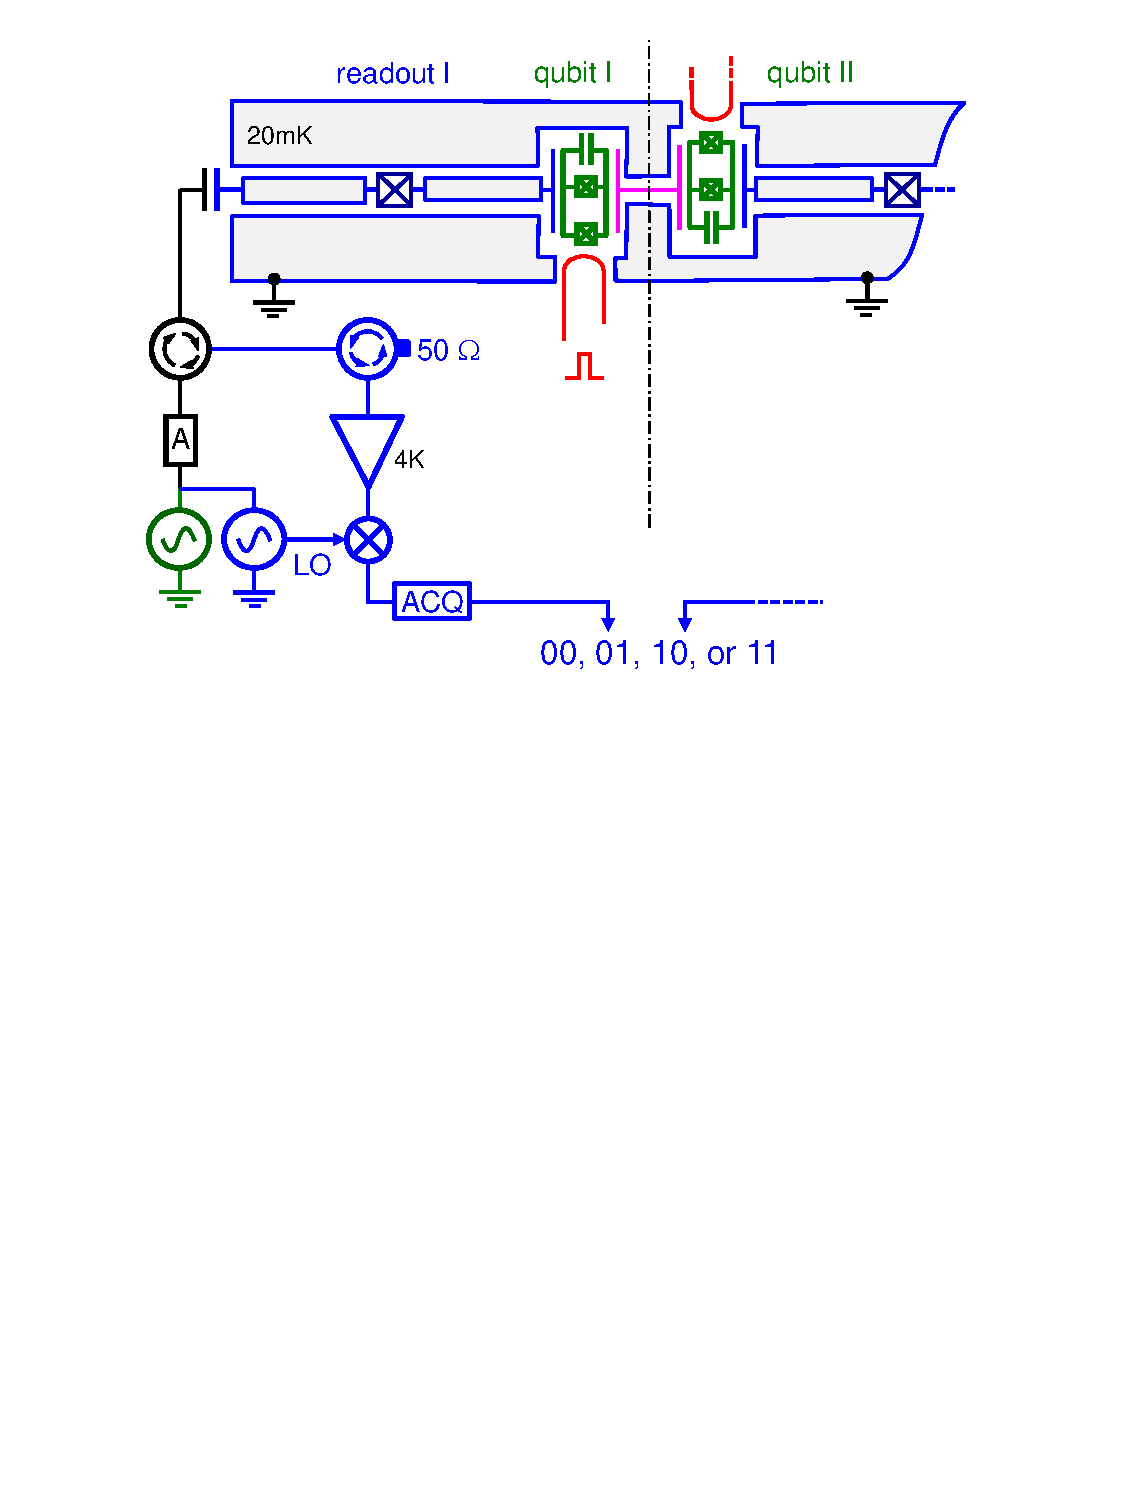
\includegraphics[width=0.75\textwidth]{./material/papers/grover/figures/2_qubit_processor_schematic}
	\caption[Circuit schematic of the realized two-qubit processor]{Circuit schematic of the two-qubit processor realized in this work, showing the two qubits in green, the qubit readouts in blue and the fast flux lines in red. Each qubit is embedded in its own nonlinear readout resonator and can be driven and read out through an individual microwave line.}
	\label{fig:two_qubit_processor_schematic}
\end{figure}

The quantum processor implemented in this work is shown in fig. \ref{fig:two_qubit_processor_schematic}. It consists of two superconducting quantum bits of the Transmon-type, each equipped with its own drive and readout circuit. The qubit readout is realized by using a nonlinear coplanar-waveguide resonator which serves as a cavity bifurcation amplifier (CBA)\citep{vijay_invited_2009} and implements a single-shot readout of the qubit state. Each qubit can be manipulated by driving it with microwave pulses through its readout resonator, allowing robust and fast single-qubit operations. The qubit frequencies can be tuned individually by fast flux lines, which allows to change the frequency each qubit over a range of several GHz. The coupling between the two qubits is realized through a fixed capacitance that connects the two top-electrodes of the qubits and implements a fixed $\sigma_{xx}$-type qubit-qubit coupling. This coupling allows us to implement a two-qubit gate and to generate entangled two-qubit states. We use this simple processor to test Bell's inequality, implement an universal two-qubit gate and perform a simple quantum algorithm that demonstrates probabilistic quantum speed-up, as will be discussed in the following sections.

\section{Demonstrating Simultaneous Single-Shot Readout}

\begin{figure}[ht!]
	\centering
		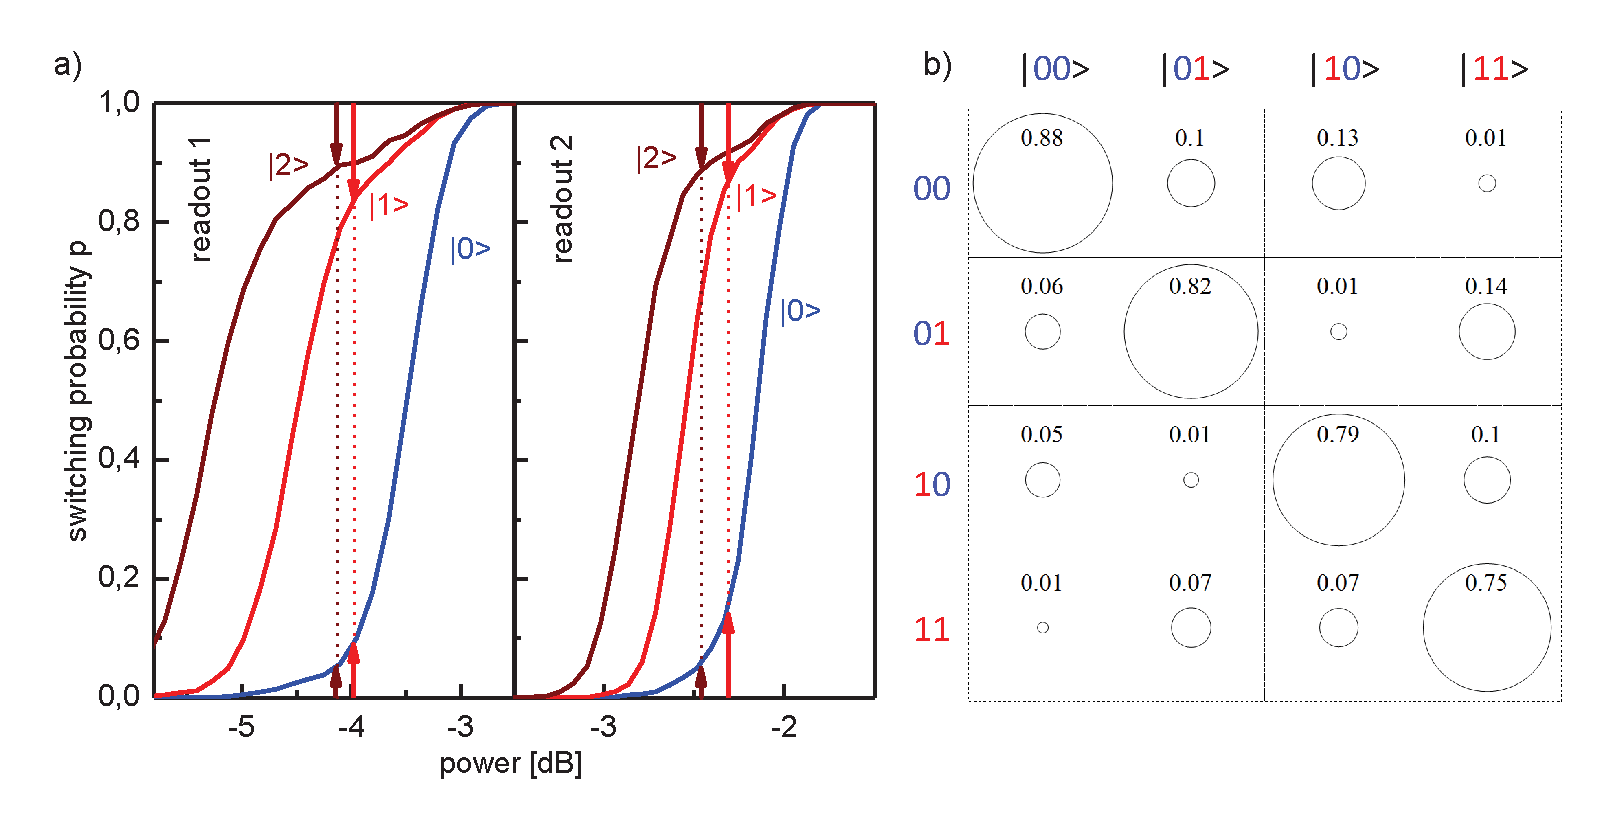
\includegraphics[width=1.\textwidth]{./material/papers/grover/figures/simultaneous_readout_characteristics}
	\caption[Switching probabilities of the two qubit readouts as a function of the readout excitation power]{a) Switching probabilities of the two qubit readouts as a function of the readout excitation power. The measurement is performed after preparing the qubits in the states $\color{blue}{\ket{0}}$, $\color{red}{\ket{1}}$ and $\color{brown}{\ket{2}}$. The readout fidelity is given as the difference in probability between the curves corresponding to the states $\color{blue}{\ket{0}}$ and $\color{red}{\ket{1}}$ or $\color{brown}{\ket{2}}$, respectively. The highest readout fidelites of 88 and 89 \% are achieved when the qubit is in state $\color{brown}{\ket{2}}$. b) Readout matrix of the two-qubit system. The matrix contains the probabilities of obtaining a given measurement result after having prepared the system in a given state. \figcomment{Replace this figure since it is not very intuitive. It would be better to show something which allows the reader to directly quantify the visibility and readout crosstalk present in the system.}}
	\label{fig:qubit_readout_characteristics}
\end{figure}

To read out the state of each qubit, a so-called cavity bifurcation amplifier \citep{siddiqi_dispersive_2006,mallet_single-shot_2009} is used. This readout technique works by capacitively coupling the qubit to a coplanar waveguide resonator which is rendered nonlinear by a Josephson junction placed in its center conductor. This nonlinear resonator can exhibit hysteretic behaviour for certain drive parameters, which can be used to map the state of the qubit to one of the bistable states of the resonator, thereby obtaining a single-shot readout. Contrary to other CQED approaches, in our setup each qubit is fitted with an individual CBA readout, allowing thus a simultaneous measurement of the full two-qubit register and therefore following closely the canonical blueprint of a quantum computer as formulated by DiVincenzo.\todo{discuss more details of the readout here...} Readout fidelitis up to 93 \% have been demonstrated using the CBA readout technique \citep{mallet_single-shot_2009} but due to design contraints only  83-85 \% fidelity have been attained in our experiments. The full characterization of the two-qubit readout is shown in fig. \ref{fig:qubit_readout_characteristics}. Fig. \ref{fig:qubit_readout_characteristics}a shows the so-called s curves of each qubit readout, which shown the working-point dependent switching probabilities of each readout with the qubits in different states. Fig. \ref{fig:qubit_readout_characteristics}b shows the full readout matrix, which connects readout switching probabilities with qubit state occupation probabilities and allows for the correction of all readout errors.

\section{Generating and Characterizing Entanglement}

\begin{figure}
	\centering
		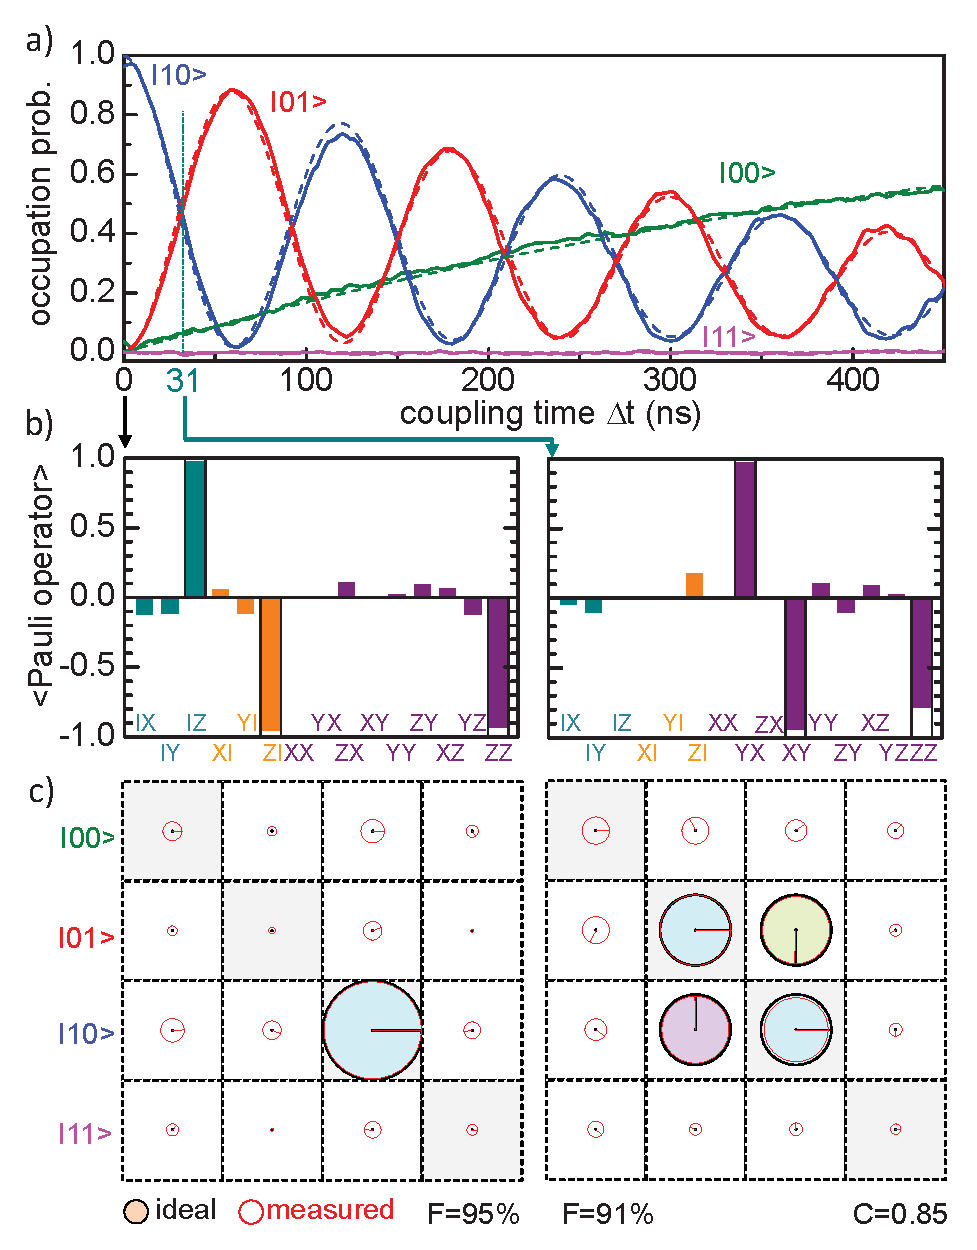
\includegraphics[width=0.7\textwidth]{./material/papers/iswap/submission1/Dewes_Figure2}
	\caption[Generating entangled two-qubit states by swapping interaction]{Energy oscillations between the two qubits induced by a resonant swapping interaction between them. a) The qubit state after switching on the swapping interaction for a given time $\Delta t$. The frequency of the oscillations corresponds to $2g = 8.7 \; \mathrm{MHz}$. b) The Pauli set of the two-qubit state measured at $0\; \mathrm{ns}$ and $31\; \mathrm{ns}$. c) The reconstructed density matrices corresponding to the two measured Pauli sets. In c), the area of each circle corresponds to the absolute value of each matrix element and the color and direction of the arrow give the phase of each element. The black circles correspond to the density matrices of the ideal states $\ket{10}$ and $1/\sqrt{2}/(\ket{10}+i\ket{01})$, respectively.\figcomment{verify sign!}}
	\label{fig:swap_interaction_state_tomography}
\end{figure}

The fixed coupling between the two qubits provides a $\sigma_{xx}$-type coupling which is only effective when the qubit frequencies are nearly resonant. Therefore, it can be switched on and off by changing the qubit frequencies, which we use to implement two-qubit gates with this system. In our processor, the effective coupling constant $g$ of the two qubits is given as $2g = 8.2 \; \mathrm{MHz}$\todo{Check if this is really $2g$!}. When using a fast fluxline pulse to abruptly tune the qubits in resonance we can switch on the qubit-qubit coupling non-adiabatically and generate an evolution operator of the form

\begin{equation}
	U(t)  =  \left( \begin{array}{cccc} 1 & 0 & 0 & 0 \\ 0 & \cos{2 \pi t g} & i\sin{2 \pi t g} & 0 \\ 0 & i\sin{2 \pi t g} & \cos{2 \pi t g} & 0 \\ 0 & 0 & 0 & 1 \end{array} \right) \label{eq:swap_evolution_operator}
\end{equation}

%explain that we stop the evolution at the right time to generate entangled states and implement a Two-qubit gate.

Switching off this interaction after a time $t_{\pi/2} = 1/8 g$ allows the creation of entangled qubit states and the implementation of a universal quantum gate, as will be explained later. Before doing this, we characterize the evoluation of the qubits during the swapping interaction by preparing them in the state $\ket{10}$, switching on the interaction for a given amount of time and measuring the qubit state directly afterwards. The resulting curve shown in fig. \ref{fig:swap_interaction_state_tomography} shows energy oscillations between the two qubits. Stopping the interaction after quarter of a period we obtain an entangled two-qubit Bell-type state that we can characterize by performing quantum state tomography. The experimental reconstruction of the density matrix of such a state corresponding approximating to the Bell-state $\ket{\psi} = 1/\sqrt{2}(\ket{01}+i\ket{10})$ is shown in fig. \ref{fig:swap_interaction_state_tomography}b. The measured fidelity of this state of 91 \% and the concurrence of 85 \% confirms that entanglement is present in the system. This entanglement can also be characterized by measuring the so-called {\it Clauser-Horne-Shimony-Holt} operator \citep{clauser_proposed_1969} on the produced state. This operator is given as

\begin{equation}
\mathrm{CHSH} = \mathrm{QS}+\mathrm{RS}+\mathrm{RT}-\mathrm{QT}
\end{equation}
with the operators $\mathrm{Q,R,S,T}$ being given as

\begin{eqnarray}
	\begin{array}{cccccccc}
		\mathrm{Q} & = & \sigma_z^1 &&& \mathrm{S} & = & \sigma_z^2\cdot \cos{\phi}+\sigma_x^2 \cdot \sin{\phi} \\
		\mathrm{R} & = & \sigma_x^1 &&& \mathrm{T} & = & -\sigma_z^2\cdot \sin{\phi}+\sigma_x^2 \cdot \cos{\phi}
	\end{array}
\end{eqnarray} 
Here, the angle $\phi$ is a parameter that should be chosen in accordance to the phase of the Bell state on which the operator is applied.

\begin{figure}[ht!]
	\centering
		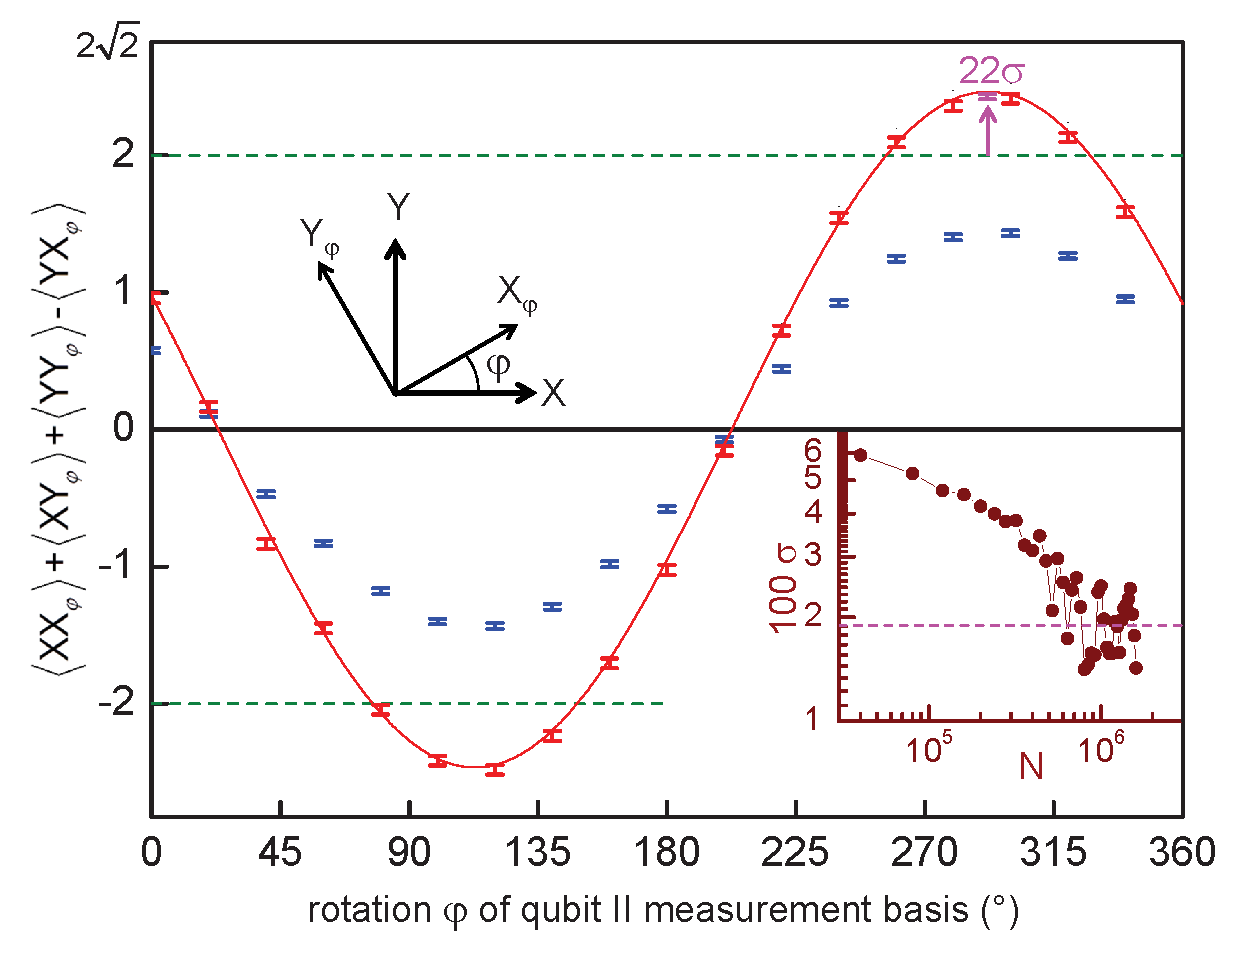
\includegraphics[width=0.7\textwidth]{./material/papers/iswap/submission1/Dewes_Figure3}
	\caption[Measurement of the CHSH operator of an entanged two-qubit state]{Measurement of the CHSH equation for an entangled two-qubit state. The renormalized CHSH expectation value (red points) exceeds the classical boundary of $2$ by a large amount. The raw measurement data (blue points) lies below this critical threshold. The inset shows the standard deviation $\sigma$ at the highest point of the curve as a function of the measurement sample size. For the highest sample count, the classical boundary is exceeded by $22$ standard deviations.\figcomment{p. 140 in cavities 6 labbook}}
	\label{fig:chsh_measurement}
\end{figure}

The expectation value $\bracket{CHSH}$ provides a test of the quantum-mechanical character of the generated state. For classical states, the maximum value is $\le 2$ but for entangled states it can reach a maximum value of $\sqrt{2}\cdot 2$. The result of a CHSH-type measurement performed on a state created by the method described above is shown in fig. \ref{fig:chsh_measurement}, showing the value of $\bracket{CHSH}$ as a function of $\phi$. We observe a violation of the classical boundary $2$ of the operator by $22$ standard deviations when correcting readout errors present in our system. However, the raw, uncorrected data fails to exceed the non-classical bound, making it impossible to close the detection loophole with our system. Nevertheless the observed violation of the equation by the renormalized state is a strong indication of entanglement in the system.

\section{Realizing a Universal Two-Qubit Quantum Gate}

\begin{SCfigure}[][ht!]
		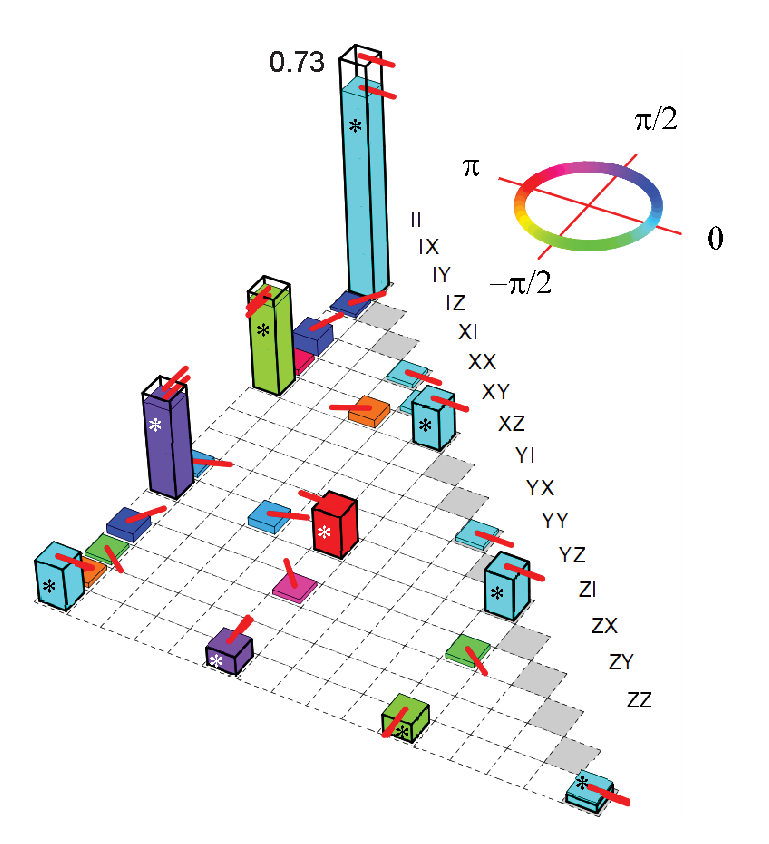
\includegraphics[width=0.65\textwidth]{./material/papers/iswap/figures/chi_matrix}
	\caption[Measured $\chi$-matrix of the $\sqrt{i\textrm{SWAP}}$ gate]{The measured $\chi$-matrix of the implemented $\sqrt{i\mathrm{SWAP}}$ gate. The row labels correspond to the indices of the $E_i$ operators, the height of each bar to the absolute value of the corresponding matrix element and the color and direction of the red arrow to the complex phase of each element. The ideal $\chi$-matrix of the $i\sqrt{\mathrm{SWAP}}$ gate is given by the outlined bars. The upper half of the positive-hermitian matrix is not shown.}
	\label{fig:gate_chi_matrix_and_errors}
\end{SCfigure}

The swapping evolution according to eq. (\ref{eq:swap_evolution_operator}) allows the implementation of a two-qubit gate. When switching on this interaction for $t_{\pi/2} = 1/8g$ we can realize the so-called $\sqrt{i\mathrm{SWAP}}$ gate, which has the representation

\begin{equation}
	\sqrt{i\mathrm{SWAP}}  =  \left( \begin{array}{cccc} 1 & 0 & 0 & 0 \\ 0 & 1/\sqrt{2} & i/\sqrt{2} & 0 \\ 0 & i/\sqrt{2} & 1/\sqrt{2} & 0 \\ 0 & 0 & 0 & 1 \end{array} \right) \label{eq:sqrt_iswap_gate}
\end{equation}
and is a universal two-qubit quantum gate. The operation and errors of our implementation of this gate can be characterized by performing quantum process tomography, yielding a gate fidelity of 90 \% . The 10 \% error in gate fidelity is caused mainly by qubit relaxation and dephasing during the gate operation and only marginally by deterministic preparation errors, as will be discussed in the main text of the thesis. Fig. \ref{fig:gate_chi_matrix_and_errors} show the measured $\chi$ matrix of the implemented gate. The achieved fidelity of the gate operation is sufficient to allow the implementation of a simple quantum algorithm with our processor, as will be discussed in the following section.
 
\section{Running a Quantum-Search Algorithm}

\begin{figure}[ht!]
	\centering
		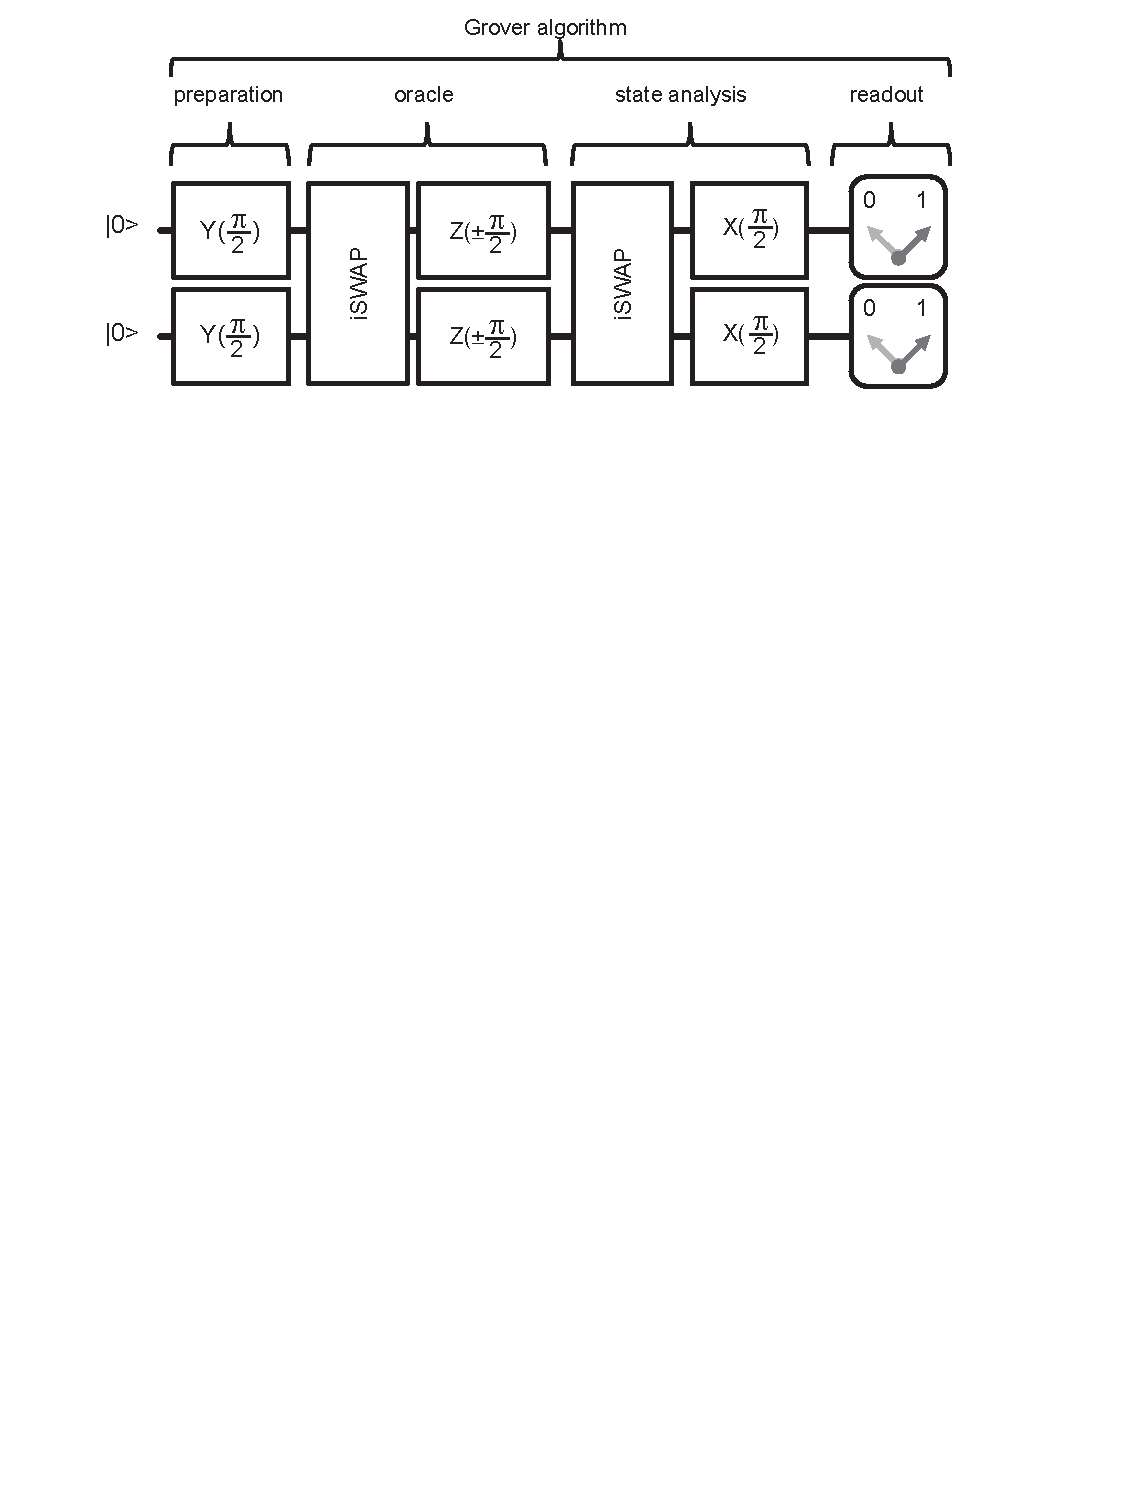
\includegraphics[width=0.8\textwidth]{./material/papers/grover/figures/grover_algorithm_schematic}
	\caption[Schematic of the implementation of Grovers search algorithm]{Schematic of the implementation of Grovers search algorithm on a two-qubit quantum processor. The algorithm consists in preparing a probe state, applying the quantum oracle to this state and analyzing the resulting output state to extract the information on the oracle operator.} 
	\label{fig:grover_algorithm_schematic}
\end{figure}

In this work we use the quantum gate implemented above to run a compiled version of Grover's search algorithm \citep{Grover_Quantum_1997}. The implemented version of the algorithm works in the basis of two qubits $x_i \in \{\ket{00},\ket{01},\ket{10},\ket{11}\}$ and  can distinguish between four different {\it oracle functions} $f(x)$ that each tag on one of the basis states $x_j$. Since the Grover algorithm for 2 qubits requires only one evaluation of the function $f(x)$ to determine which state has been marked it is faster than any conceivable classical algorithm, thus demonstrating the concept of quantum speed-up. The schematic of our version of Grover's algorithm is shown in fig. \ref{fig:grover_algorithm_schematic} and involves two $i\mathrm{SWAP}$ gates and three single-qubit operations along with a single-shot qubit readout at the end of the algorithm. We implemented all steps of this algorithm with our two-qubit processor and performed quantum state tomography after each step to reconstruct the quantum state at different points in the algorithm. Fig. \ref{fig:grover_density_matrices_state_1} shows the experimentially measured density matrices when running the algorithm with an oracle that marks the state $\ket{00}$. State tomographies are shown after applying the generalized Hadamard transform, after applying the quantum oracle and after the final step of the algorithm. This reconstruction of the quantum state using quantum state tomography does not however allow to demonstrate quantum speed-up, which requires individual single-shot readout of the qubit register, which will be discussed in the following section.

\begin{figure}[ht!]
	\centering
		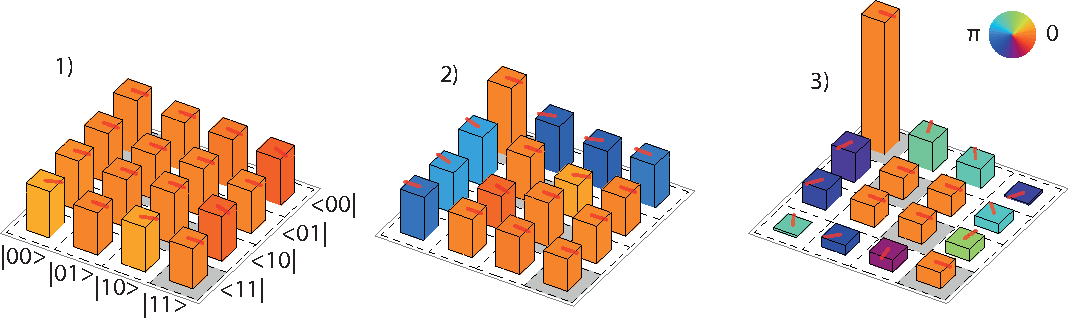
\includegraphics[width=1.\textwidth]{./material/figures/2-qubit-processor/grover/grover-density-matrices-state-1}
	\caption[Measured density matrices when running Grover's algorithm]{Measured density matrices when running Grover's search algorithm with a search oracle marking the state $\ket{00}$. 1) shows the state after the generalized Hadamard transform, 2) after applying the quantum oracle and 3) after the final step of Grover's algorithm.} 
	\label{fig:grover_density_matrices_state_1}
\end{figure}


\section{Demonstrating Quantum Speed-Up}

The main interest of running a quantum algorithm is to obtain an advantage in the run-time in comparision with a classical algorithm, the so-called {\it quantum speed-up}. To characterize this quantum speed-up as obtained with our processor, we run Grovers algorithm for all four possible oracle functions and directly readout out the qubit state after the last step of the algorithm, without correcting any readout errors. When averaging the results of such individual runs of the algorithm we can then obtain its single-run fidelity, which --for our processor-- ranges between 52 and 67 \%, depending on the state which is  marked by the quantum oracle, as shown in fig. \ref{fig:grover_single_shot_probabilities}. These results clearly demonstrate quantum speed-up in this system, although the achieved success probability is considerably lower than the theoretically possible value of 100 \% . The reduced fidelity is mainly due to relaxation and decoherence of the qubit state during the running of the algorithm and to a very small degree due to errors in the pulse sequence and drifts in the measurement equipment.

\begin{figure}[ht!]
		\centering
		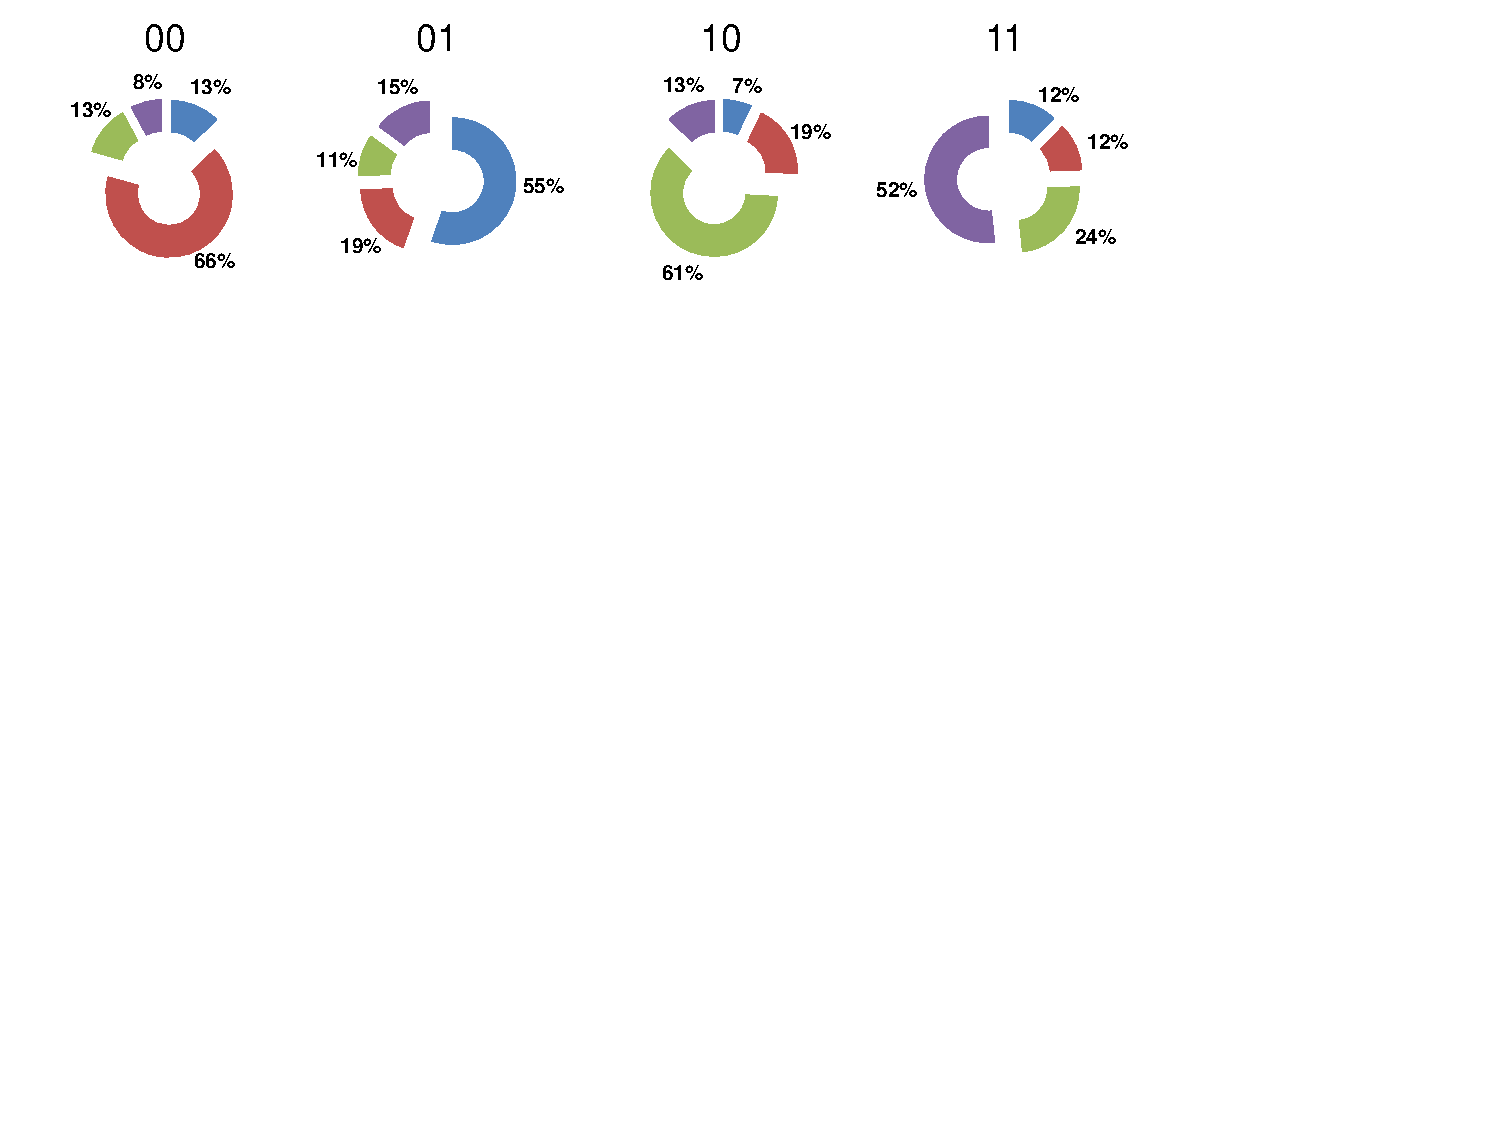
\includegraphics[width=1.0\textwidth]{./material/papers/grover/figures/grover_algorithm_single_shot_probabilities}
	\caption[Single-run results of the Grover search algorithm]{Single-run results when running the Grover search algorithm on our two-qubit quantum processor. Shown are the probabilities of obtaining the results $00,01,10,11$ as a function of the oracle function provided to the algorithm, indicated by the number on top of each graph. In all four cases, the success probability of the algorithm is $> 50 \%$, thus outperforming any classical algorithm in the number of calls to the oracle function.}
	\label{fig:grover_single_shot_probabilities}
\end{figure}

\section{Designing a Scalable Quantum Computing Architecture}

After having demonstrated the different building blocks of a superconducting, Transmon-based quantum processor it remains to be shown that larger-scale quantum-computing beyond two qubits is possible with this system. This work therefore pursued the realization of a more scalable qubit architecture using systems of up to six qubits coupled through a so-called ``quantum bus'' \citep{majer_coupling_2007}. The details of this novel architecture are discussed in the following sections.

The approach for scalable quantum computing with superconducting qubits pursued in this work consists of a system of many individual Transmon qubits equipped with individual JBA-based readouts, a multiplexed drive and readout circuit and a fixed qubit-qubit coupling mediated through a high-Q CPW resonator. As before, each qubit possesses a fluxline for fast frequency control. The readout and drive signals are send to all the qubits in parallel through a multiplexed transmission line. In this approach, the qubit and readout parameters, couplings and frequencies have to be carefully to avoid unwanted coupling between individual qubits and readouts and to allow the implementation of robust quantum gates between individual qubits. In this work we realized a 4-qubit chip and characterized it experimentally. The results of these experiments will be discussed in the main text of this thesis.

\begin{figure}[ht!]
  \centering
	\includegraphics[width=1.\textwidth]{"./material/figures/scalable-architecture/scalable architecture - schematic"}
	\caption[...]{...}
\end{figure}


%-A Two-Qubit Quantum Processor
%-Building Blocks: Single Qubit Gates, Qubit Readout, Two-Qubit Gate
%-Implementation
%-Frequency Tunability of the Qubits
%  -Decoherence Times
%-Characterization of the Readout
%  -Readout Errors
%-Single Qubit Gates: Tune-Up & Characterization
%-2 Qubit Gate: Tune-Up & Characterization
%-Tests of Entanglement
%  -Entanglement Witnesses
%  -Bell's Inequality
%-2 Qubit Algorithms
%-Grover's Search Algorithm:
%   -Introduction & Background
%   -Implementation
%   -Measurements
%   -Error Analysis
%   -Conclusions

\chapter{Realizing a Two-Qubit Processor}

This chapter discusses the main experimental results of this thesis. We start by discussing the implementation of a superconducting two-qubit processor, discussing the characteristics of the Transmon qubits used in the processor, the readout scheme, single-qubit manipulation, two-qubit gates as well as the experimental procedures used for quantum state and quantum process tomography. The last section of this chapter will discuss the implementation of a quantum algorithm -- so called Grover search algorithm -- using our two-qubit processor and the demonstration of quantum speed-up achieved with our system.

%-Discuss all the experiments performed during the PhD thesis.

\section{Introduction \& Motivation}

\begin{figure}[ht!]
  \centering
	\includegraphics[width=1.\textwidth]{"./material/figures/2-qubit-processor/processor schematic"}
	\caption[Circuit schematic of the two-qubit processor]{The circuit schematic of the two-qubit processor used in this work. Shown are the two Transmon qubits in green, the drive and readout circuit in blue, the fast flux lines in red and the coupling capacitance in magenta.}
	\label{fig:2_qubit_chip_circuit_diagram}
\end{figure}

As discussed in the introduction, the most simple, usable quantum processor contains two qubits that are coupled by an universal two-qubit gate and which in addition can be manipulated and read out individually. We realized such a two-qubit processor using two Transmon qubits, coupled through a fixed capacitance and readout out by individual single-shot readout of the JBA type. The circuit diagram of our processor is shown in fig. \ref{fig:2_qubit_chip_circuit_diagram}, showing the qubits, the drive and readout circuit and the coupling element between them. The following sections we'll discuss the parameters of individual parts of the processor.

\begin{figure}
	\centering
		\includegraphics[width=1.\textwidth]{"./data/ct5/2011_04_11 - anticrossing/processor_spectroscopy"}
	\label{fig:ProcessorSpectroscopy}
	\caption[Spectroscopy of the Two-Qubit Processor]{Spectroscopy of the realized two-qubit processor. a) $\ket{0}\to\ket{1}$ and $(\ket{0}\to\ket{2})/2$ transition frequencies of the two qubits with fitted dependence and cavity frequencies. b) Avoided level crossing of the $\ket{01}$ and $\ket{10}$ levels of the qubits with fit, $g = 8.7 \; \mathrm{MHz}$. c) Spectroscopy of qubit 1 at the point indicated in b).}
\end{figure}

\section{Processor Design}

The parameters of the sample have been chosen in accordance to various design constraints of the qubit processor. For the qubits, the main design goals were high coherence time, good frequency tunability and fast drivability. As we will show later, the coherence time of the qubit is limited by relaxation to the ground state and coupling to external noise sources. The relaxation component of the Transmon qubit is ultimately limited by internal losses of the Josephson junction but usually is bound by coupling to the electromagnetic environment, as will be discussed later. The frequency tunability is important for the realization of fast two-qubit gates but can also limit the relaxation and coherence time of the qubit by coupling to external noise sources. The drivability speed on the other hand is limited by the anharmonicity of the qubit, which can however not be increased arbitrarily since it will make the qubit sensitive to charge noise when chosen too high. For the readout, the main design goals were readout speed and fidelity. The speed of the readout is limited by the quality factor of the readout resonator, which however also can induce qubit relaxation through the Purcell effect and may therefore not be chosen too small.

In the following paragraphs we'll therefore discuss the parameter design for our two-qubit processor and analyze the sample parameters that have been obtained.

\section{Processor Fabrication}

In this section we will discuss the fabrication of the two-qubit processor realized in this work.

\section{Measurement Setup}

\begin{figure}[ht!]
	\centering
		\includegraphics[width=1.\textwidth]{"./material/figures/2-qubit-processor/measurement setup"}
	\caption[The measurement setup used for the two-qubit experiments]{The measurement setup used for the two-qubit experiments. Exactly the same drive and readout scheme is used for both qubits with phase-locked microwave sources and arbitrary waveform generators.}
	\label{fig:MeasurementSetup}
\end{figure}

Fig. \ref{fig:MeasurementSetup} show the measurement setup used for the two-qubit experiments. We use the following components along the measurement chain to generate, mix and read out microwave and DC signals:

\begin{itemize}
\item \textit{Qubit microwave pulses}: We use two continous-wave microwave generators that generate phase-locked single-frequency microwave tones which are used for driving the two qubits. These pulses are mixed with fast control pulses generated by an arbitrary waveform generators (Tektronix AWG5014b) using a passive Hittite IQ mixer. By using sideband mixing in the frequency range of 0-300 MHz we can generate multi-frequency drive pulses with arbitrary frequency and phase shift in respect to the drive tone. The IQ mixer exhibits frequency-dependent amplitude and phase errors which are measured using a fast spectrum analyzer (Rhode \& Schwarz FSP series) and corrected by adapting the AWG waveform fed to the mixer (see Appendix).
\item \textit{Flux pulses}: We use a second pair of AWGs to generate the flux drive pulses of each qubit. These pulses are attenuated by 20 dB and filtered using both conventional microwave low-pass filters as well as a pair of absorptive custom-made Eccosorb microwave filters, which exhibit a very high attenuation up to UHF frequencies (see Appendix for more details) \todo{add exact link!}. The flux signal is fed back to room temperature through an identical piece of transmission line, which permits the measurement and compensation of the signal distortion caused by the response function of the transmission line (see Appendix for more details) \todo{add exact link!}.
\item \textit{Readout pulses}: We use a pair of continuous-wave microwave generators (Anritsu MG3692B) to generate a single-frequency pump tone which is mixed with a pulse shape signal generated by an arbitrary function generator (Tektronix AFG6352), fed through a tunable attenuator and combined with the qubit drive pulses. The readout pulses typically possess a rise time of 30 ns, a hold time of 200 ns and a latch time of about 2 $\mu$s at 90 \% of the hold height.
\item \textit{Drive and measurement line}: The combined drive and readout signals are attenuated by 70 dB on their way to the qubit chip, where they are reflected and sent back through an output line connected to the input by a cryogenic circulator (PAMTECH \todo{add the exact reference here}). The reflected measurement signal gets bandpass-filtered and amplified by a cryogenic HEMT amplifier and several room-temperature amplifiers. At room temperature it gets IQ-demodulated with the original continuous microwave tone and digitized by a four-channel 4GS/s ADC card (Acqiris DC282).
\end{itemize}

\section{Measurement techniques}

In this section we will discuss the techniques used to characterize and manipulate our two-qubit processor. All techniques employed are based on ...

\section{Processor Characterization}

This section discusses the detailed characterization of individual circuit parts that will be used later to realize two-qubit gate and to run a quantum algorithm on the processor. The discussion will focus on the readout and microwave manipulation of the qubits as well as  on the reconstruction of quantum states from measurement data, which will be used later for characterizing gate and processor operation.

\subsection{Spectroscopic measurements}

The following section discusses the parameters of our two-qubit processor that have been obtained by various measurements.

\subsubsection{Qubit Parameters}

\subsubsection{Readout Parameters}

\begin{itemize}
\item \textit{Qubits}: Spectroscopic measurement of the qubit transitions yielded parameter values of $E_J^I / h = 36.2\; \mathrm{GHz}$, $E_c^I / h = 0.98 \; \mathrm{GHz}$ and $E_J^{II} / h = 43.1\; \mathrm{GHz}$, $E_C^{II} / h = 0.87 \; \mathrm{GHz}$ for the Josephson and charging energies of the two qubits and values of $d^I = 0.2$, $d^{II} =  0.35$ for the qubit junction asymmetries.
\item \textit{Readout resonator}: The frequencies of the readout resonators have been measured as $\nu_R^I = 6.84 \; \mathrm{GHz}$ and $\nu_R^{II} = 6.70 \; \mathrm{GHz}$ with quality factors $Q^I \simeq Q^{II} = 730$, independent measurements of the Kerr nonlinearities yielded $K^I / \nu_R^I \simeq K^{II} / \nu_R^{II} = -2.3\pm 0.5 \times 10^{-5}$ \todo{add junction parameters inferred from the bare resonator frequencies}.
\item \textit{Qubit-Resonator coupling}: The coupling of the qubits to the readout resonators has been spectroscopically determined as $g_0^I \simeq g_0^{II} = 50 \; \mathrm{MHz}$
\end{itemize}

\subsection{Readout}

%-Discuss the readout errors and crosstalk

\subsection{Single-Qubit Operations}

%-Discuss single qubit manipulation, gate fidelity and state tomography
%Data: 14/12/2010


%discuss calibration of mixers, sideband pulses etc.

\begin{figure}
	\centering
		\includegraphics[width=1.\textwidth]{"./data/ct5/2010_12_01 - iq tomography/iq_tomographies"}
	\label{fig:SingleQubitIQControl}
	\caption{}
\end{figure}

%
\subsection{Quantum State Tomography}

Quantum state tomography is the procedure of experimentally determining an unknown quantum state\citep{michael_a._nielsen_quantum_2000}.

The density matrix of an n-qubit system can be written in general form as
\begin{eqnarray}
\rho & = & \sum\limits_{v_1,v_2\hdots v_n} \frac{c_{v_1,v_2\hdots v_n} \sigma_{v_1}\otimes \sigma_{v_2}\hdots \sigma_{v_n}}{2^n} \label{eq:state_tomography_state_representation} \\
c_{v_1,v_2\hdots v_n} & = & \mathrm{tr}\left(\sigma_{v_1}\otimes \sigma_{v_2}\hdots \otimes\sigma_{v_n} \; \rho \right)  \label{eq:state_tomography_coefficients}
\end{eqnarray}
where $v_i \in \left\{ X,Y,Z,I\right\}$ and $n$ gives the number of qubits in the system and where the $c_{v_1,v_2\hdots v_n}$ are real-valued coefficients that fully describe the given density matrix. To reconstruct the density matrix of an experimental quantum system in a well-prepared state it is therefore sufficient to measure the expectation values of these $n^2-1$ coefficients on an ensemble of identically prepared systems. However, statistical and systematic measurement errors can yield a set of coefficients that corresponds to a {\it non-physical} density matrix which violates either the positivity or unity-trace requirement. In the following paragraph we will therefore discuss a technique with which one can estimate the density matrix of a system in a more correct way.

\subsubsection{Maximum Likelihood Estimation}

A method which is often used in quantum state tomography is the so-called {\it maximum-likelihood} technique. Rather than directly calculating the density matrix of the system from the obtained expectation values $c_{v_1,v_2\hdots v_n}$, it calculates the joint probability of measuring a set $\{c_{X,X,\hdots,X},c_{Y,X,\hdots,X},\hdots,c_{I,I,\hdots,I}\}$ for a given estimate of the density matrix $\hat{\rho}$. By numerically or analytically maximizing this joint probability over the set of possible density matrices we obtain the density matrix which is most likely to have produced the set of measurement outcomes that we have observed.

The joint measurement operators $\Sigma_j = \sigma_{v_1}\otimes \sigma_{v_2}\hdots \otimes\sigma_{v_n}$ have the eigenvalues $\pm 1$ and can thus be written as 
\begin{equation}
\sigma_{v_1}\otimes \sigma_{v_2}\hdots \otimes\sigma_{v_n} = \ket{+_j}\bra{+_j}-\ket{-_j}\bra{-_j}
\end{equation}
where $\ket{-_j}$ and $\ket{-_j}$ are the eigenstates corresponding to the eigenvalues $\pm 1$ of $\Sigma_j$. The expectation value $\langle \Sigma_j \rangle$ can be estimated by the quantity
\begin{equation}
\widehat{\langle \Sigma_j \rangle}_\rho = \frac{1}{l}\sum\limits_{i = 1}^l M_i(\Sigma_j,\rho) \label{eq:tomography_measurement_estimator}
\end{equation}
 where $M_i(M,\rho)$ denotes the outcome of the $i$-th measurement of the operator $M$ on the state described by the density matrix $\rho$. This quantity is binomially distributed with the expectation value $E(\widehat{\langle \Sigma_j \rangle}_\rho) = \langle \Sigma_j \rangle_\rho$ and the variance $\sigma^2(\widehat{\langle \Sigma_j \rangle}_\rho) = 1/l \cdot (1-\langle \Sigma_j \rangle_\rho^2)$. For large sample sizes $l$, the binomial distribution can be well approximated by a normal distribution with the same expectation value and variance. The joint probability of obtaining a set of measurement values $\{s_1,\hdots,s_{n^2-1}\}$ for the set of operators $\{\widehat{\langle\Sigma_1 \rangle}_\rho,\hdots,\widehat{\langle\Sigma_{n^2-1} \rangle}_\rho\}$ is then given as
\begin{equation}
P\left(\widehat{\langle \Sigma_1 \rangle }_\rho = s_1;\hdots;\widehat{\langle \Sigma_{n^2-1} \rangle}_\rho =  s_{n^2-1}\right) = \prod\limits_{i = 1}^{n^2-1} \exp{\left(-\frac{l}{2}\frac{(s_i-\langle \Sigma_i \rangle_\rho)^2}{1-\langle \Sigma_i \rangle_\rho^2}\right)}
\end{equation}
By maximizing this probability (or the logarithm of it) we obtain an estimate of the density matrix $\rho$ of the quantum state. This technique also allows us to include further optimization parameters when calculating the joint probability. This is useful for modeling e.g. systematic errors of the measurement or preparation process, which can be described by modifying the operators contained in the probability sum. A common source of errors in our tomography measurements are errors in the microwave pulses used to drive the qubit. Since our measurement apparatus permits us only to measure the $\sigma_z$ operator of each qubit we have to perform $\pi/2$ rotations about the $Y$ or $-X$ axes of the Bloch sphere of each individual qubit in order to measure the values of the $\sigma_x$ and $\sigma_y$ operators, which we therefore replace with an effective measurement of each qubits $\sigma_z$ operator preceded by a rotation $R_{\nu_i}$ given as
\begin{eqnarray}
R_{X} & = & \exp{\left( -i \sigma_y \pi / 4\right)} \\
R_{Y} & = & \exp{\left( +i \sigma_x \pi / 4\right)} 
\end{eqnarray}
Phase and amplitude errors can be modeled as
\begin{eqnarray}
R_{X} & = & \exp{\left( -i \left[+\sigma_y\cos{\alpha}+\sigma_x\sin{\alpha} \right] \left[\pi / 4+\gamma\right]\right)} \\
R_{Y} & = & \exp{\left( +i \left[-\sigma_y\sin{\beta}+\sigma_x\cos{\beta}\right] \left[\pi / 4+\delta\right]\right)} 
\end{eqnarray}
Here, $\alpha$ and $\beta$ represent phase errors whereas $\gamma$ and $\delta$ represent amplitude errors in the drive pulses.

\subsection{Two Qubit Operations}

\subsubsection{Creation of Entanglement}

\begin{figure}
	\centering
		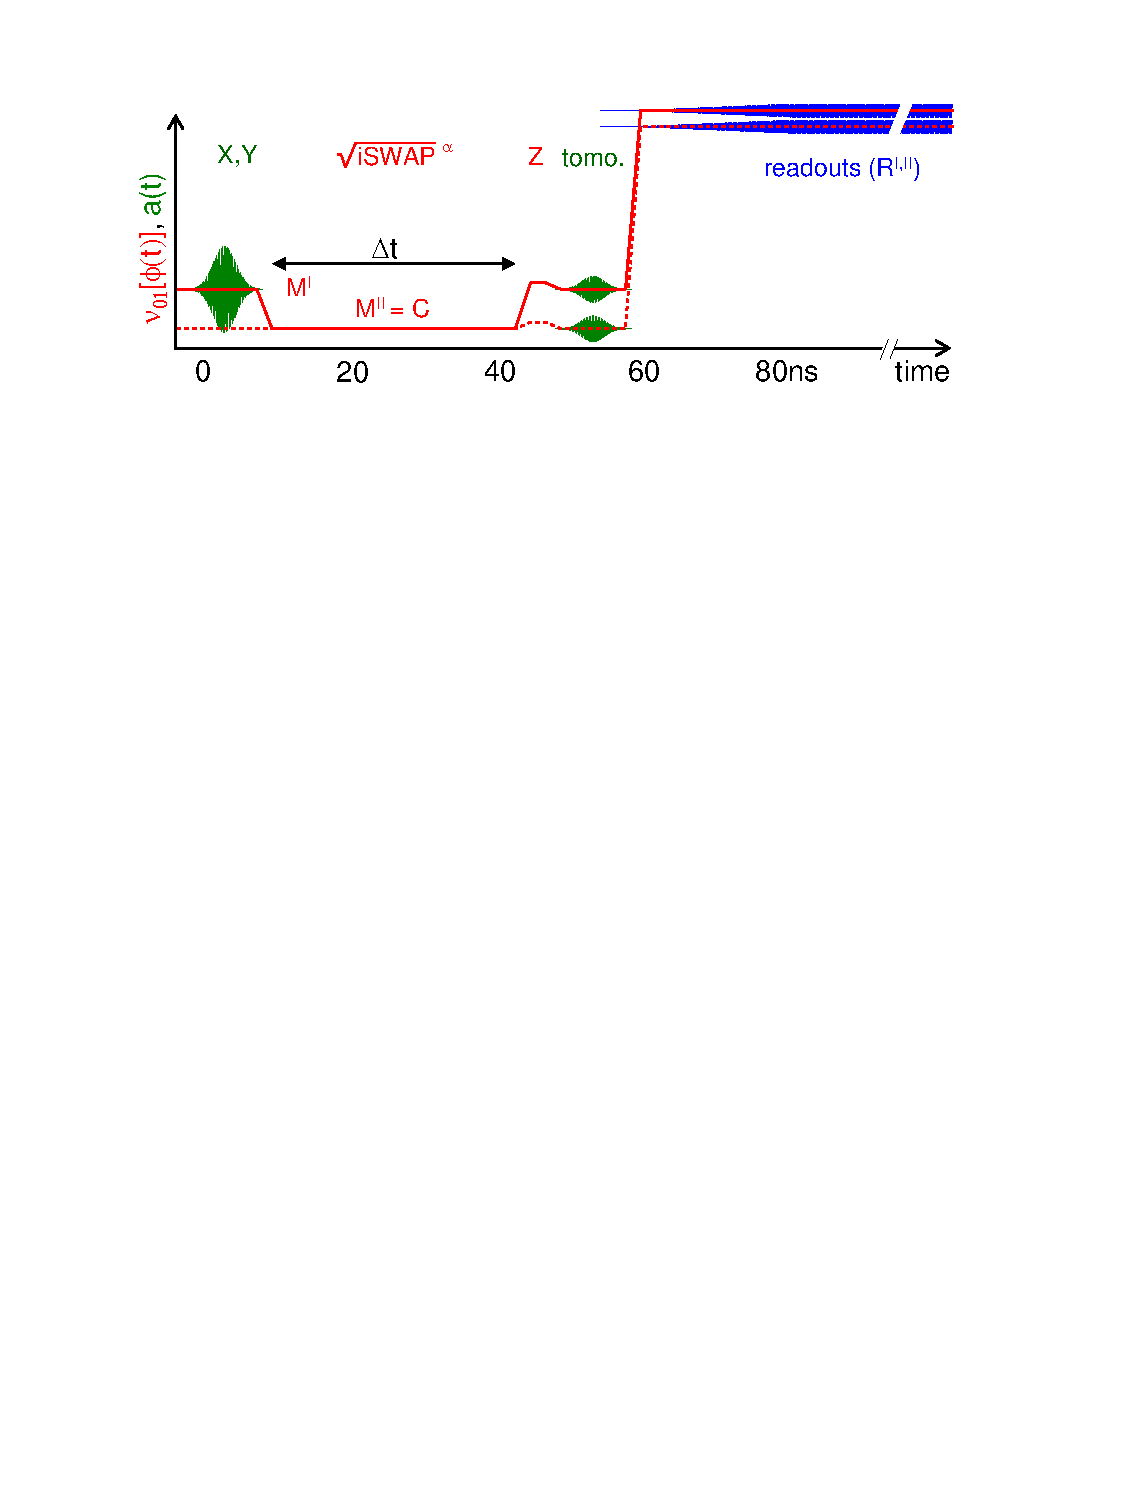
\includegraphics[width=0.8\textwidth]{./material/papers/iswap/figures/iswap_gate_pulse_sequence}
	\label{fig:ISwapPulseSequence}
	\caption{}
\end{figure}

\subsubsection{Violation of Bell's inequality}

\begin{figure}
	\centering
		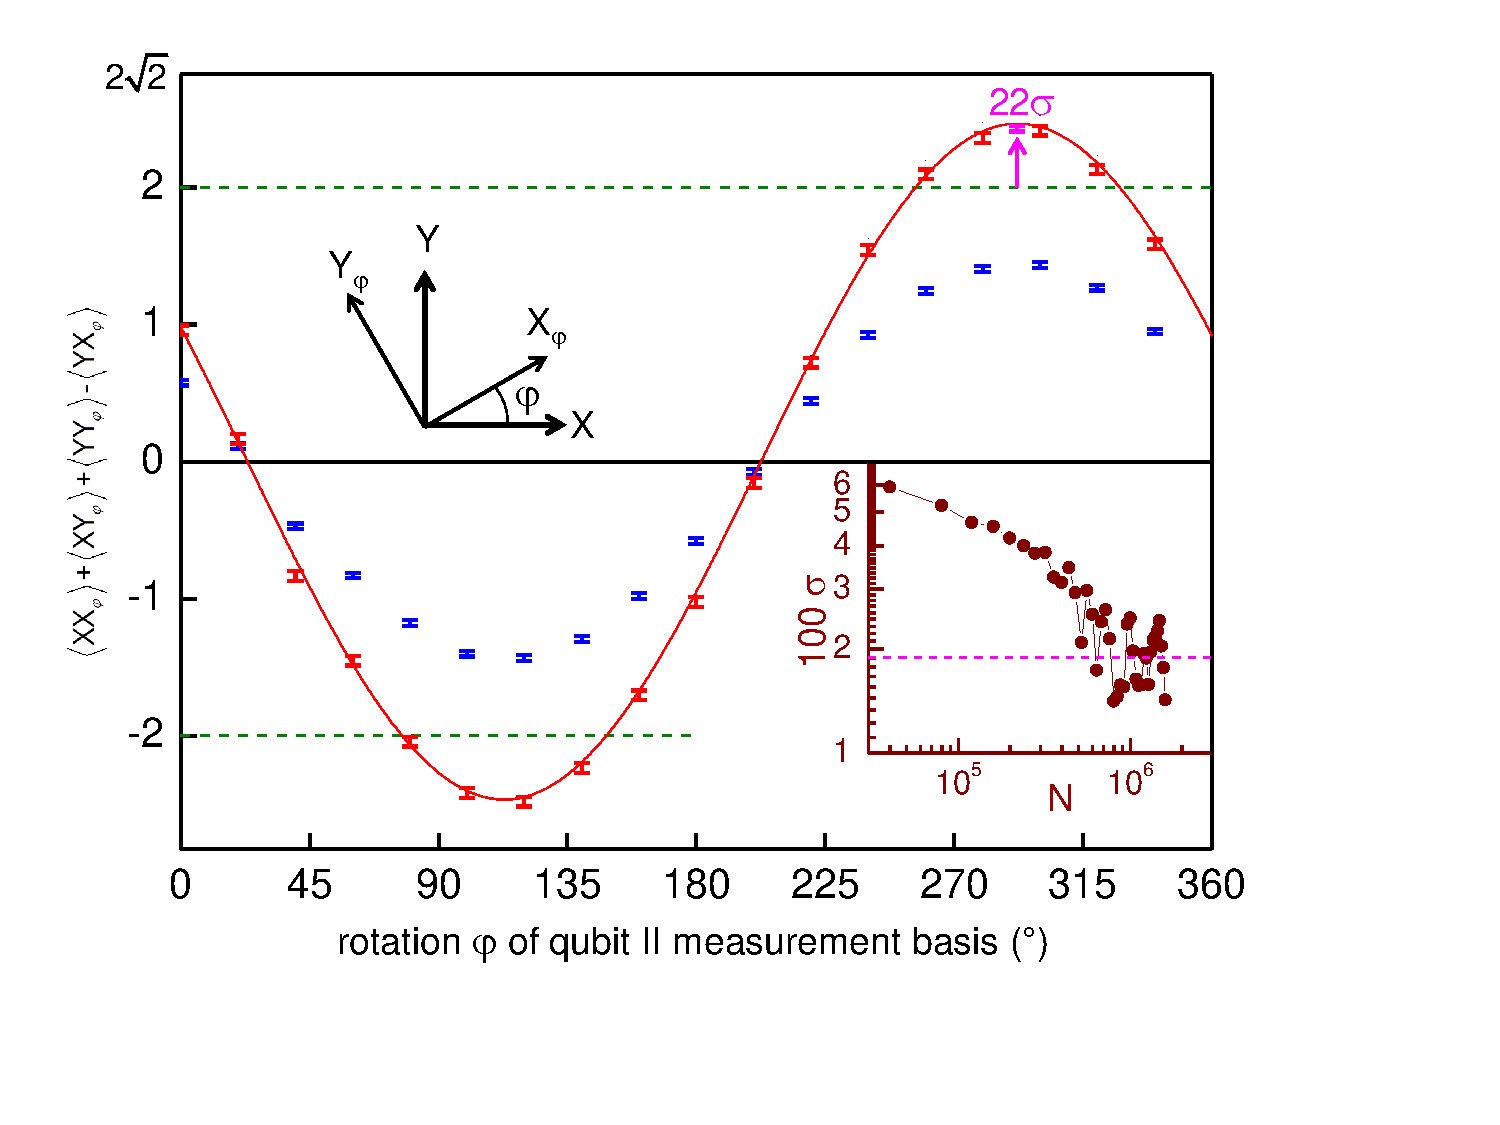
\includegraphics[width=0.8\textwidth]{./material/papers/iswap/figures/chsh}
	\label{fig:CHSH}
	\caption{}
\end{figure}

\subsection{Characterizing Quantum Processes}

\subsubsection{Introduction \& Principle}

\subsubsection{Implementation}

A quantum process can be described as a map $\mathcal{E} : \rho_\mathcal{H} \to \rho_\mathcal{H}$ that maps a density matrix $\rho$ defined in a Hilbert space $Q_1$ to another density matrix $\mathcal{E}(\rho)$ defined in a target Hilbert space $Q_2$ and fulfilling three axiomatic properties \cite{michael_a._nielsen_quantum_2000,haroche_exploring_2006}:

\begin{axiom}
$\mathrm{tr}\left[\mathcal{E}(\rho)\right]$ is the probability that the process represented by $\mathcal{E}$ occurs, when $\rho$ is the initial state.
\end{axiom}

\begin{axiom}
$\mathcal{E}$ is a {\it convex-linear map} on the set of density matrices, that is, for probabilities $\left\{p_i\right\}$,

  \begin{equation}
	  \mathcal{E}\left(\sum\limits_i p_i \rho_i\right) = \sum\limits_i p_i \mathcal{E}(\rho_i)
	\end{equation}
\end{axiom}

\begin{axiom}
$\mathcal{E}$ is a {\it completely-positive} map. That is, if $\mathcal{E}$  maps density operators of system $Q_1$ to density operators of system $Q_2$, then $\mathcal{E}(A)$ must be positive for any positive operator $A$. Furthermore, if we introduce an extra system $R$ of arbitrary dimensionality, it must be true that $(\mathcal{I}\otimes \mathcal{E})(A)$ is positive for any positive operator $A$ on the combined system $RQ_1$, where $\mathcal{I}$ denotes the identity map on system $R$.
\end{axiom}
As shown in \cite{michael_a._nielsen_quantum_2000}, any quantum process fulfilling these criteria can be written in the form

\begin{equation}
  \mathcal{E}(\rho) = \sum\limits_i E_i \rho E_i^\dagger \label{eq:process_operator_sum_representation}
\end{equation}
for some set of operators $\{ E_i \}$ which map the input Hilbert space to the output Hilbert space, and $\sum_i E_i^\dagger E_i \le I$.

Now, if we express the operators $E_i$ in a different operator basis $\tilde{E}_j$ such that $E_i = \sum_j a_{ij} \tilde{E}_{j}$ and insert into eq. (\ref{eq:process_operator_sum_representation}), we obtain

\begin{eqnarray}
 \mathcal{E}(\rho) & = & \sum\limits_i \sum\limits_j a_{ij} \tilde{E}_j \;\rho\; \sum\limits_k a_{ik}^* \tilde{E}_k^\dagger \\
& = & \sum\limits_{j,k}\tilde{E}_j \; \rho \; \tilde{E}_k^\dagger \sum\limits_i a_{ij} a_{ik}^* \\
& = & \sum\limits_{j,k}\tilde{E}_j \; \rho \; \tilde{E}_k^\dagger \; \chi_{jk} \label{eq:process_chi_representation}
\end{eqnarray}
where we defined $\chi_{jk} = \sum\limits_i a_{ij} a_{ik}^*$. This is the so-called $\chi$-matrix representation of the quantum process. Here, all the information on the process is contained in the $\chi$ matrix, which controls the action of the process-independent operators $\tilde{E}_i$ on the initial density matrix $\rho$.

Now, the goal of {\it quantum process tomography} is to obtain the coefficients of the $\chi$-matrix -- or any other complete representation of the process -- from a set of experimentally measured density matrices $\rho$ and $\mathcal{E}(\rho)$.

To achieve this, several techniques have been developed. The technique used in this work is the so-called {\it standard quantum process tomography (SQPT)}. This technique proceeds as follows:

\begin{enumerate}
\item Choose a set of operators $E_i$ that forms a full basis of $\mathcal{M}: Q_1 \to Q_2$. For n-qubit process tomography we usually choose $E_{i_1,i_2 \hdots i_n} = \sigma_{i_1}\otimes \sigma_{i_2}\hdots\otimes\sigma_{i_n}$, where $\sigma_i$ are the single-qubit Pauli operators and $i\in\{I,X,Y,Z\}$. 
\item Choose a set of pure quantum states $\ket{\phi_i}$ such that $\ket{\phi_i}\bra{\phi_i}$ span the whole space of input density matrices $\rho$. Usually, for a n-qubit system we choose $\phi = \{\ket{0},\ket{1},(\ket{0}+\ket{1})/\sqrt{2},(\ket{0}+i\ket{1})/\sqrt{2}\}^{\otimes n}$, where $^{\otimes n}$ denotes the n-dimensional Kronecker product of all possible permutations.
\item For each of the $\ket{\phi_i}$, determine $\mathcal{E}(\ket{\phi_i}\bra{\phi_i})$ by quantum state tomography. Usually we also determine $\ket{\phi_i}\bra{\phi_i}$ experimentally since the preparation of this state already entails small preparation errors that should be taken into account when performing quantum process tomography. 
\end{enumerate}

After having obtained the $\rho_i$ and $\mathcal{E}(\rho_i)$ one obtains the $\chi$-matrix by writing $\mathcal{E}(\rho_i) = \sum_j \lambda_{ij} \tilde{\rho}_j$, with some arbitrary basis $\tilde{\rho}_j$ and
letting $\tilde{E}_m \tilde{\rho}_j \tilde{E}_n^\dagger = \sum_k \beta_{jk}^{mn}\tilde{\rho}_k$. We can then insert into eq. (\ref{eq:process_chi_representation}) and obtain
\begin{eqnarray}
\sum\limits_k \lambda_{ik} \tilde{\rho}_k & = & \sum\limits_{m,n} \chi_{mn} \sum\limits_k \beta_{ik}^{mn} \tilde{\rho}_k  
\end{eqnarray}
This directly yields $\lambda_{ik} = \sum_{m,n}\beta_{ik}^{mn}\; \chi_{mn}$, which, by linear inversion,  gives $\chi$.

\subsubsection{The Kraus representation}

Besides the $\chi$-matrix representation, there is another useful way of expressing a quantum map, the so called {\it Kraus representation}, which is given as

\begin{equation}
 \mathcal{E}(\rho) = \sum\limits_i M_i \; \rho \; M_i^\dagger \label{eq:process_kraus_representation}
\end{equation}

It can be shown \citep{haroche_exploring_2006} that this sum contains at most $N$ elements, where $N$ is the dimension of the Hilbert space of the density matrix $\rho$. We can go from the $\chi$ representation to the Kraus representation by changing the basis $\tilde{E}_i$ such that

\begin{equation}
	\tilde{E}_i = \sum\limits_l a_{il}\; \breve{E}_l
\end{equation}

which, for eq. (\ref{eq:process_chi_representation}), yields

\begin{eqnarray}
 \mathcal{E}(\rho) & = & \sum\limits_{j,k} \sum\limits_l a_{jl} \breve{E}_l \; \rho \sum\limits_m a_{km}^* \breve{E}_m^\dagger \; \chi_{jk} \\
 & = & \sum\limits_{l,m}  \breve{E}_l \; \rho \; \breve{E}_m^\dagger \; \sum\limits_{j,k} a_{jl} a_{km}^* \chi_{jk} \label{eq:process_chi_transformed}
\end{eqnarray}

The last sum on the right side of eq. (\ref{eq:process_chi_transformed}) corresponds to a change of coordinates of the matrix $\chi$. Now, we can pick the $a$ such that $\chi$ is diagonal in the new basis $\breve{E}$ and obtain

\begin{eqnarray}
 \mathcal{E}(\rho) & = &  \sum\limits_{l} \lambda_l \breve{E}_l \; \rho \; \breve{E}_l^\dagger \\
& = &  \sum\limits_{l} M_l \; \rho \; M_l^\dagger
\end{eqnarray}
with $\lambda_l$ being the $l$-th eigenvalue of the $\chi$ matrix with the eigen-operator $\breve{E}_l$ and $M_{l} = \sqrt{\lambda_l} \breve{E}_l$.


\subsection{Realizing a Two-Qubit Gate}

\begin{figure}
   \centering
	 \includegraphics[width=1.\textwidth]{"./data/ct5/film of swap/pauli_set_vs_time_with_simulation"}
	 \caption[test]{testcaption}
	 \label{fig:swap_pauli_set_vs_time_with_simulation}
\end{figure}

\subsubsection{Principle}

\subsubsection{Implementation}

\subsubsection{Fidelity}

\subsubsection{Error Analysis}

%-Discuss the realization of a 2 qubit gate:
%  -Principle
%  -Implementation & Pulse Sequency
%  -Characterization through Quantum Process Tomography:
%     -Principles: State tomography, Pauli set, process tomography
%     -Discuss alternative representations of the process information:
%        -Chi matrix, Choi matrix, S, log S, Kraus operator representation
%  		-Errors: Discuss simulations, error models and possible reasons for discrepancies

\begin{figure}
	\centering
		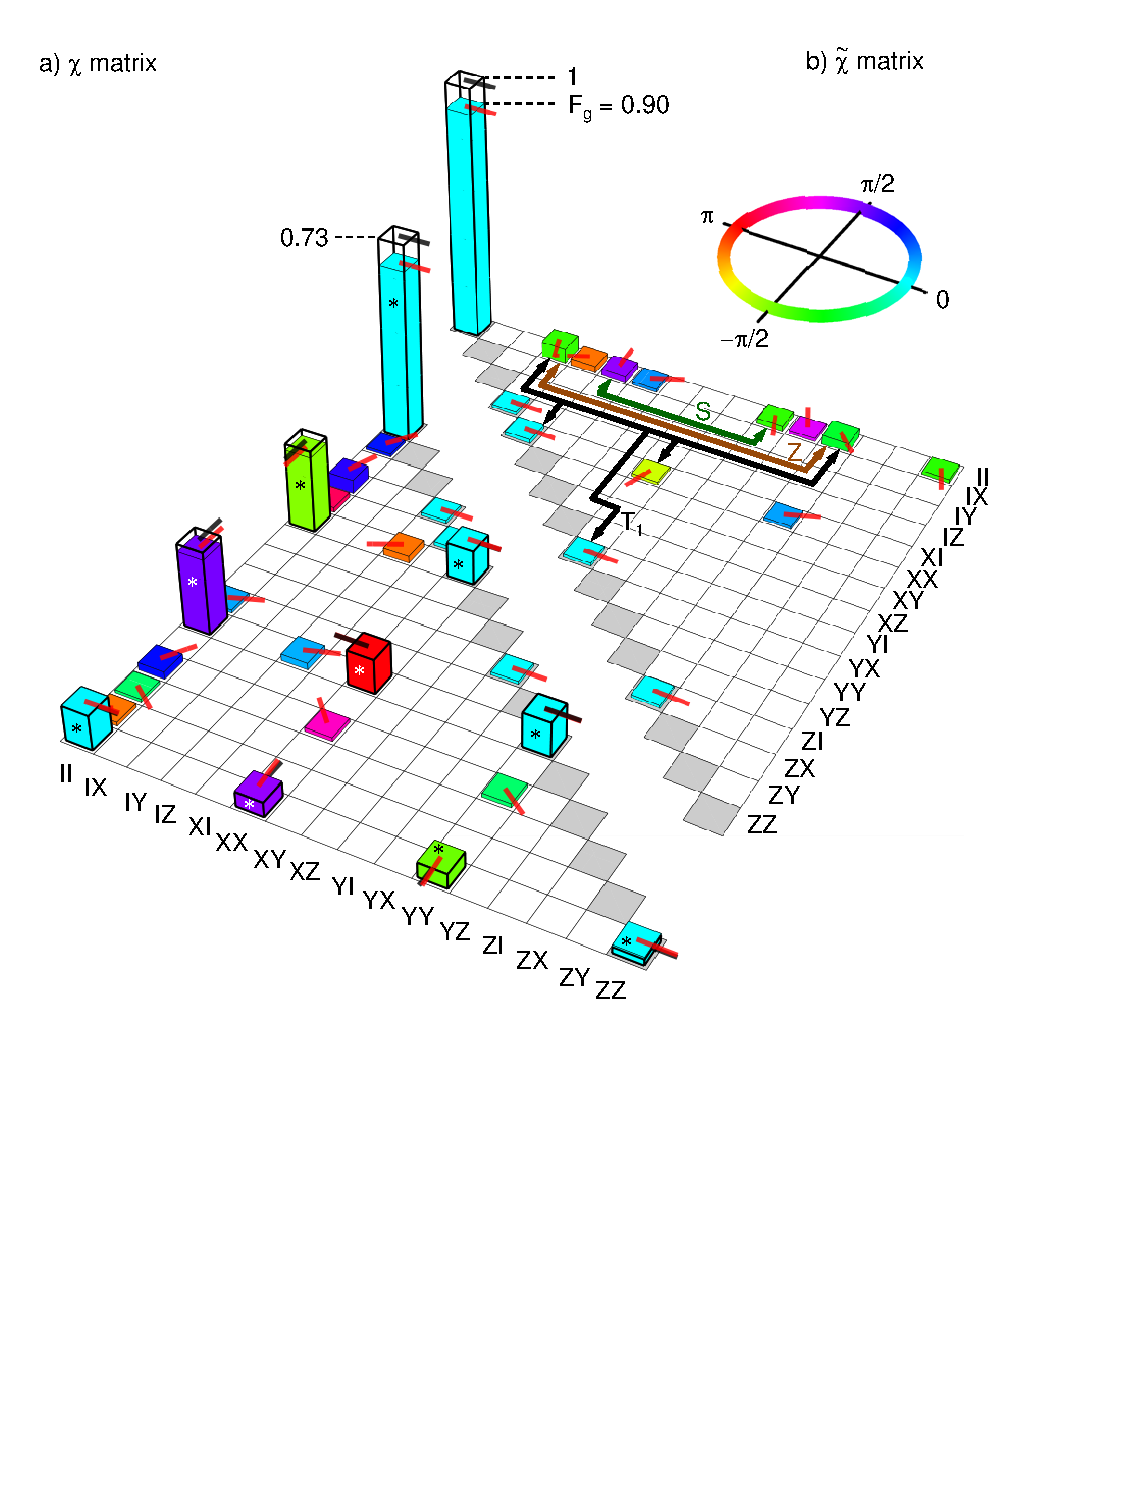
\includegraphics[width=1.\textwidth]{./material/papers/iswap/figures/chi_matrix_and_error_process}
	\label{fig:GateChiMatrixAndErrorProcess}
	\caption{}
\end{figure}


\section{Running Grover's Search Algorithm}

%Motivate this experiment:
% -Benchmark for superconducting quantum computers
% -Speed-up for searching in an unsorted database

\begin{figure}
	\centering
		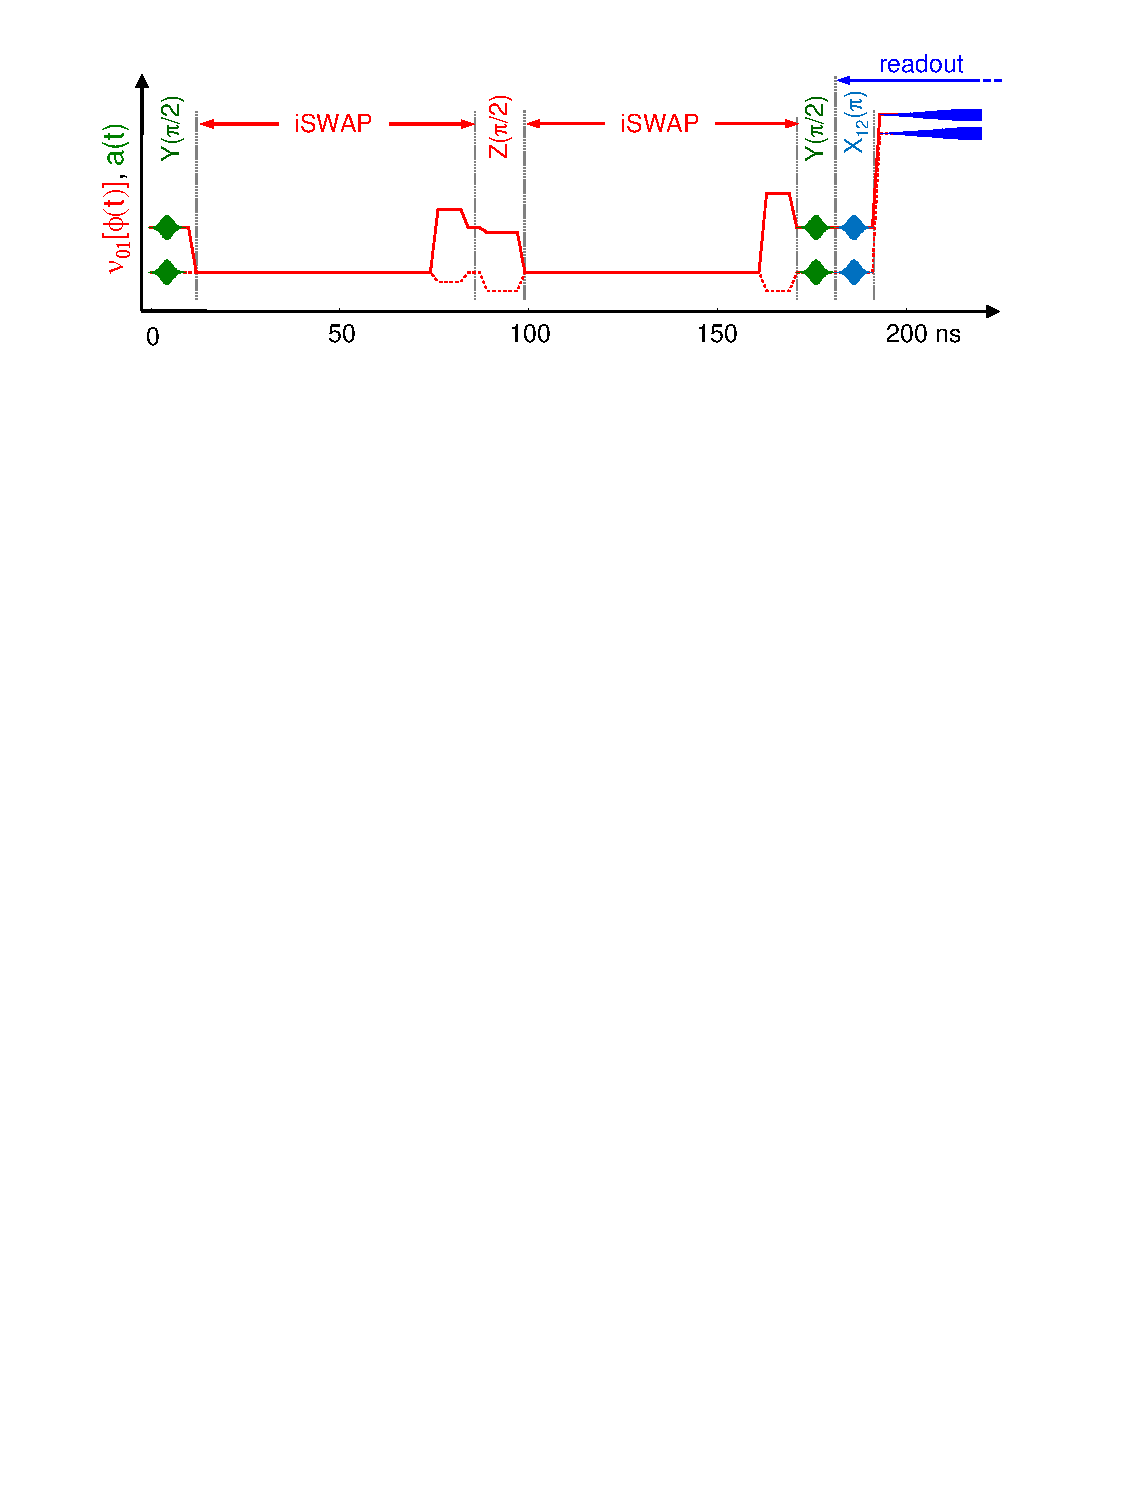
\includegraphics[width=1.\textwidth]{./material/papers/grover/figures/grover_algorithm_pulse_sequence}
	\label{fig:Grover3}
	\caption[Pulse sequence used for implementing Grovers search algorithm]{The pulse sequence used in realizing Grover's quantum search algorithm. First, a $Y_{\pi/2}$ pulse is applied to each qubit to produce the fully superposed state $1/2(\ket{00}+\ket{01}+\ket{10}+\ket{11})$. Then, an $i\mathrm{SWAP}$ gate is applied, followed by a $Z_{\pm \pi /2}$ gate on each qubit, which corrsponds to the application of the oracle function. The resulting state is then analyzed using another $i\mathrm{SWAP}$ gate and two $Y_{\pi/2}$ gates to extract the state which has been marked by the oracle function. Optionally, a $Y^{12}_{\pi}$ pulse is used on each qubit to increase the readout fidelity.}
\end{figure}

\subsection{Introduction \& Motivation}

\begin{enumerate}
  \item {\textbf Inputs:} An oracle function $\mathcal{O}$ which performs the operation $O\ket{x}\ket{q} = \ket{x}\ket{q\otimes f(x)}$, where $f(x) = \delta_{x,x_0}$
  \item {\textbf Outputs:} The marked state $x_0$
	\item Initialize the qubit register to the state: 
	$$\ket{\psi} \to \ket{0}^{\otimes n}\ket{0}$$
	\item Apply the Hadamard transformation to all of the qubits: 
	$$\ket{psi}\to \frac{1}{\sqrt{2^n}}\sum\limits_{x=0}^{2^n-1} \ket{x} \left[ \frac{\ket{0}-\ket{1}}{\sqrt{2}} \right]$$
	\item Apply the Grover iteration $R \approx [\pi \sqrt{2^n}/4]$ times:
	$$ \ket{\psi} \to \left[(2 \ket{\psi}\bra{\psi}-I)\mathcal{O}\right]^R \frac{1}{\sqrt{2^n}} \sum\limits_{x=0}^{2^n-1}\ket{x} \left[ \frac{\ket{0}-\ket{1}}{\sqrt{2}} \right] \approx \ket{x_0}\left[\frac{\ket{0}-\ket{1}}{\sqrt{2}}\right] $$
	\item Measure the first n qubits to obtain $x_0$
\end{enumerate}

For the Two-qubit case, this algorithm can be drastically simplified -- or ``compiled'' -- such that it runs without the ancilla qubit and in one single step of the Grover iteration:

\begin{enumerate}
  \item {\textbf Inputs:} An oracle function $\mathcal{O}$ which performs the operation $O\ket{x} =(-1)^{\delta_{x,x_0}}\ket{x}$, where $x_0$ is the marked state that is searched.
  \item {\textbf Outputs:} The marked state $x_0$
	\item 
\end{enumerate}

%-Explain the Grover experiment...
%		-Theoretical interest
%		-First demonstration in NMR
%   -Potential speed-up
%   -Details of the algorithm:
%     -Elementary operations
%     -Pulse shapes, corrections, ...

\begin{figure}
	\centering
		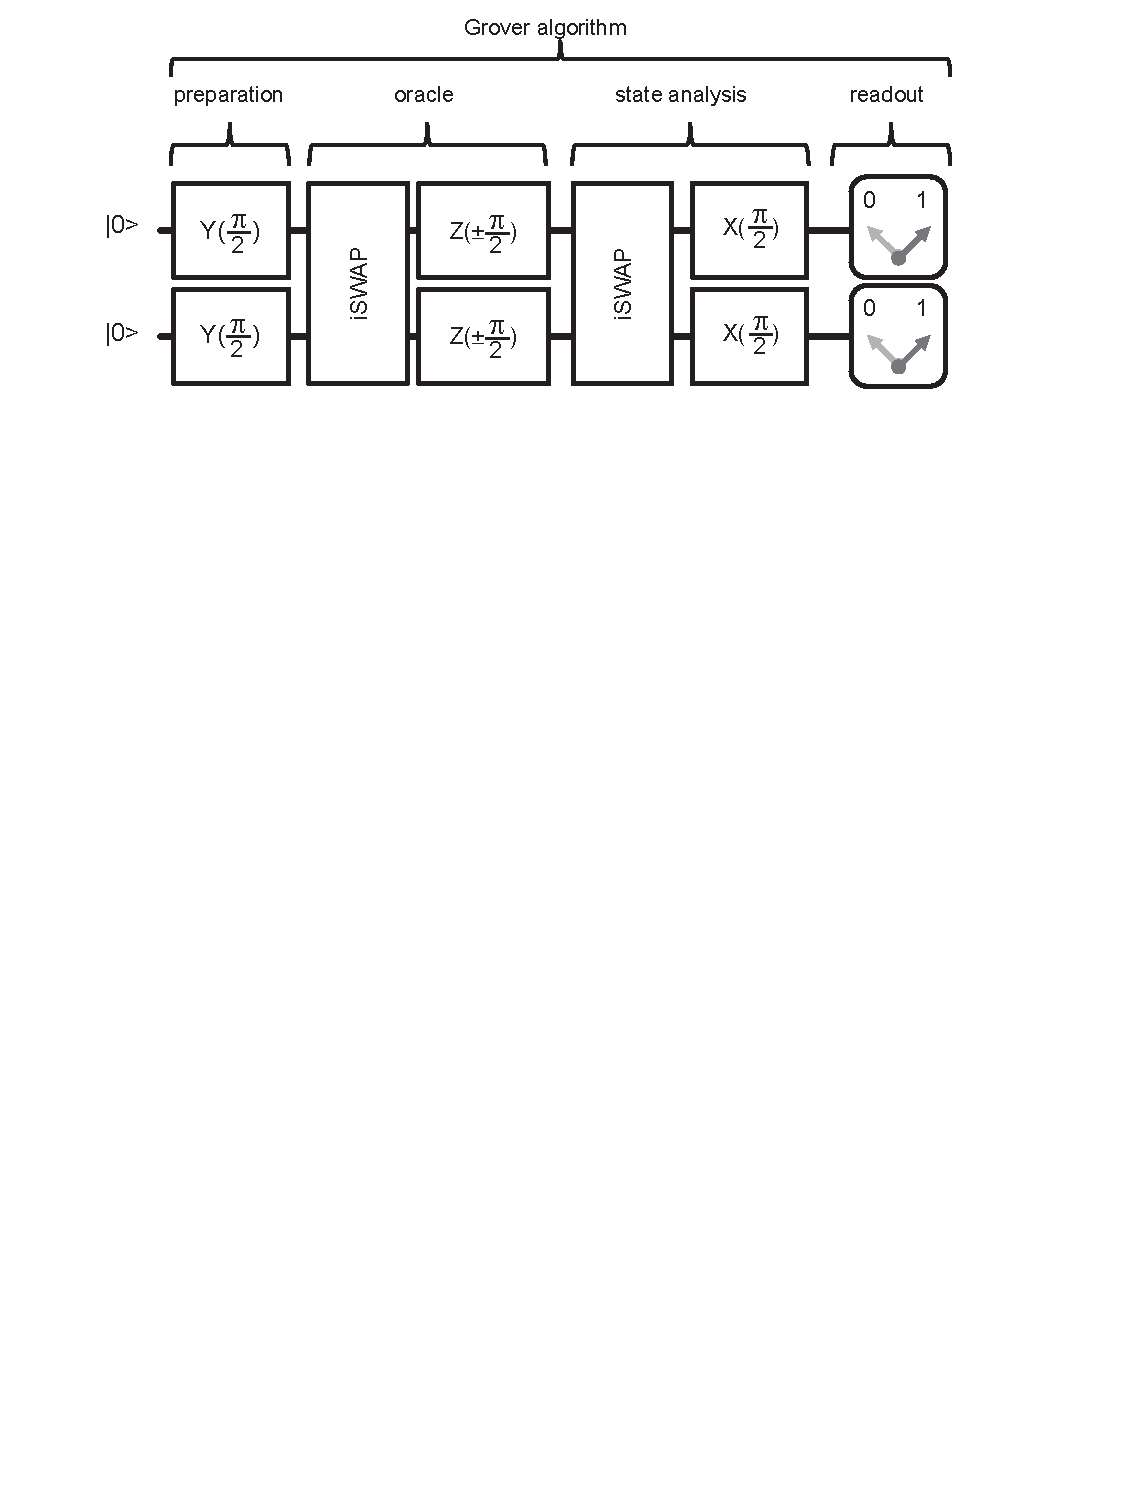
\includegraphics[width=1.\textwidth]{./material/papers/grover/figures/grover_algorithm_schematic}
	\label{fig:GroverAlgorithmSchematic}
	\caption{}
\end{figure}

\subsection{Experimental Implementation}

%-Show the implementation principle of the experiment.
%  -Break down the algorithm using the universal quantum gates that we've implemented

\subsection{Results}

%To Do:
%  -Create figures for all steps of the algorithm using Matplotlib
%  -Re-Analyze the data using Denis' Mathematica
%-Discuss the results and errors.

\begin{figure}
	\centering
		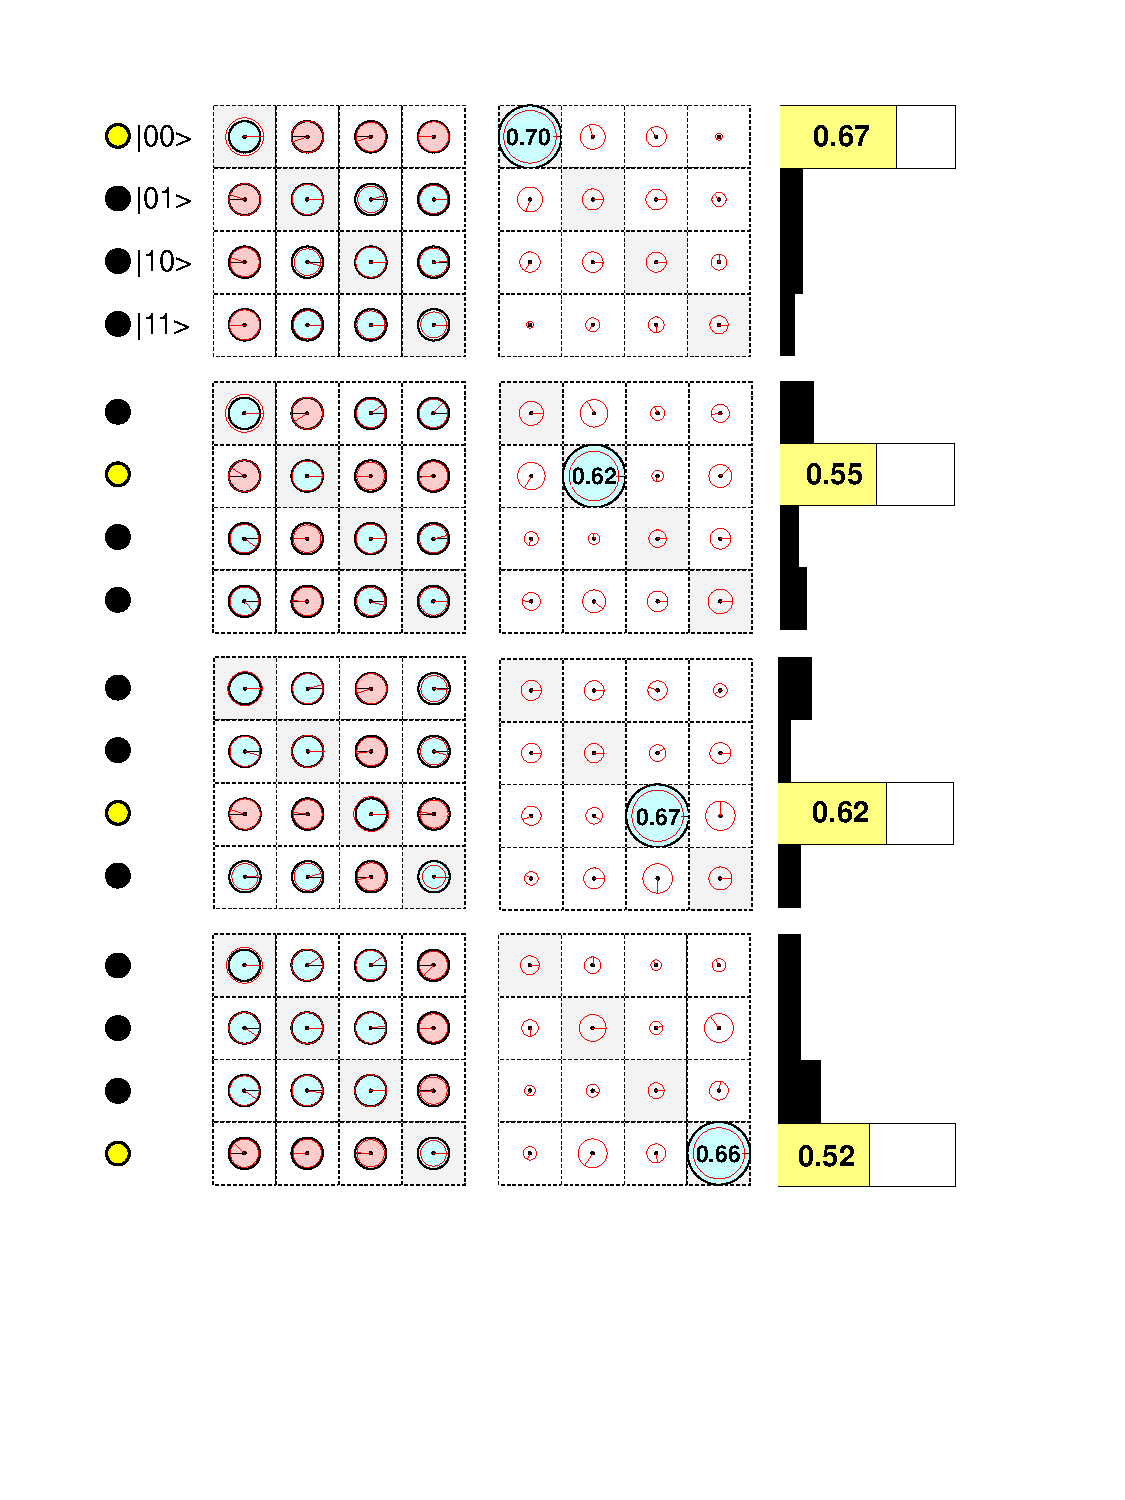
\includegraphics[width=1.\textwidth]{./material/papers/grover/figures/grover_algorithm_experimental_results}
	\label{fig:GroverAlgorithmExperimentalResults}
	\caption{}
\end{figure}

\subsubsection{Algorithm Fidelity}


\subsubsection{Single-Run Probabilities}

\subsubsection{Error Analysis}

\subsection{Conclusions}

%-Conclusions regarding quantum speed-up and applicability of results to larger-scale quantum computing.


\input{"scalable architecture"}

\chapter{Conclusions \& Outlook}

\section{Significance of Performed Experiments}

\section{Future Directions in Superconducting QC}

\subsection{3D Circuit Quantum Electrodynamics}

\subsection{Hybrid Quantum Systems}

\subsection{Quantum Error Correction}

\subsection{Quantum Feedback}


\appendix

\input{"appendix - modeling"}

\input{"appendix - data acquisition"}

\input{"appendix - fabrication"}

\bibliographystyle{apalike}

\stepcounter{chapter}

\addcontentsline{toc}{chapter}{\numberline {\thechapter} Bibliography}

\bibliography{thesis}

\end{document}
